\documentclass[12pt, twoside]{report}

%Packages and Dependencies
\usepackage[utf8]{inputenc}
\usepackage{style}

\begin{document}

%%%%%%%%%%% Half Title
\thispagestyle{empty}
\vspace*{\fill}
\begin{center}
\textsc{\Large MULTI-PLATFORM GENOMIC DATA FUSION WITH INTEGRATIVE DEEP LEARNING}
\end{center}
\vspace*{\fill}
%%%%%%%%%%%%%%%%%%%%%

\setcounter{page}{0}
\clearpage

%%%%%%%%%%% Title page 
\thispagestyle{empty}
\begin{center}
    \vfill
    \textsc{\Large MULTI-PLATFORM GENOMIC DATA FUSION WITH INTEGRATIVE DEEP LEARNING}\\
    \vfill
    By Olatunji Oni, B.Sc. \\
    \vfill
    {\large \textit{A Thesis Submitted to the School of Graduate Studies in the Partial Fulfillment of the Requirements for the Degree Master of Science}}\\

    \vfill
    {\large McMaster University\, \copyright\, Copyright by Olatunji Oni\, \today}\\[4cm]
\end{center}
%%%%%%%%%%%%%%%%%%%%%%%

\newpage
\pagenumbering{roman}
\setcounter{page}{2}

\begin{singlespace}
    \noindent
    McMaster University \\ 
    Master of Science\, (\the\year) \\
    Hamilton, Ontario (School of Computational Science and Engineering) \\[1.5cm]
    TITLE: Multi-Platform Genomic Data Fusion with Integrative Deep Learning \\
    AUTHOR: Olatunji Oni\,  %list previous degrees
    (McMaster University)  \\
    SUPERVISOR: Dr. Sanzheng Qiao\, \\ 
    NUMBER OF PAGES: \pageref{lastoffront}, \pageref{LastPage}
\end{singlespace}

\clearpage
%%%%%%%%%%%%%%%%% ABSTRACT
\section*{\Huge Abstract} 
\addcontentsline{toc}{section}{Abstract}
 %Abstract goes here
\clearpage

%%%%%%%%%%%%% ACKNOWLEDGEMENTS
\section*{\Huge Acknowledgments} 
\addcontentsline{toc}{section}{Acknowledgments}
 %Acknowledgements
\clearpage

% \begin{singlespace}
% \end{singlespace}

\frontmatter{}
    \tableofcontents
    \listoftables
    \listoffigures
    \begin{table}[ht]
\caption{Summary of Mathematical Notations} % title of Table
\centering % used for centering table
\begin{tabular}{l l} % centered columns (4 columns)
\hline %inserts single horizontal lines
Symbol & Description \\ %[0.5ex] % inserts table
%heading
\hline % inserts single horizontal line
$X$ & A matrix. \\ % inserting body of the table
$\hat{y}$ & The model approximation from a neural network.  \\
$\theta$ & The variable weights in a neural network.  \\
$b$ & The bias terms in a neural network. \\  % [1ex] adds vertical space
$\Theta$ & The set of all parameters in a neural network.  \\
$J(\cdot)$ & A neural network cost function. \\
$\psi(\cdot)$ & An activation function. \\
$\alpha$ & An optimization learning rate. \\
$\tilde{x}$ & The noised version of input data $x$.  \\
$x'$ & The reconstruction of input data $x$ from an autoencoder.  \\
$g_{\theta}(\cdot)$ & The encoding function of an autoencoder.  \\
$f_{\theta^{T}}(\cdot)$ & The decoding function of an autoencoder. \\ 
$\mathbb{Z}_{\geq 0}$ & The set of all non-negative integers. \\ [1ex]
\hline %inserts single line
\end{tabular}
\label{table:notation}
\end{table}

\label{lastoffront}
\clearpage

    
    \pagenumbering{arabic}
    \pagestyle{fancy}
    \fancyhead{}
    \fancyfoot{}
    \fancyhead[RE,LO]{McMaster University --- Comput. Sci. \& Engineering}
    \fancyhead[LE,RO]{MSc Thesis --- Olatunji Oni}
    \fancyfoot[CE,CO]{\thepage}
    
    

The abundance of next-generation sequencing (NGS) data has encouraged the adoption of machine learning methods to aid in the diagnosis and treatment of human disease. In particular, the last decade has shown the extensive use of predictive analytics in cancer research due to the prevalence of rich cellular descriptions of genetic and transcriptomic profiles of cancer cells. Despite the availability of wide-ranging forms of genomic data, few predictive models are designed to leverage multidimensional data sources. In this paper, we introduce a deep learning approach using neural network based information fusion to facilitate the integration of multi-platform genomic data, and the prediction of cancer cell sub-class. We propose the dGMU (deep gated multimodal unit), a series multiplicative gates that can learn intermediate representations between multi-platform genomic data and improve cancer cell stratification. We also provide a framework for interpretable dimensionality reduction and assess several methods that visualize and explain the decisions of the underlying model. Experimental results on nine cancer types and four forms of NGS data (copy number variation, simple nucleotide variation, RNA expression, and miRNA expression) showed that the dGMU model improved the classification agreement of unimodal approaches and outperformed other fusion strategies in class accuracy. The results indicate that deep learning architectures based on multiplicative gates have the potential to expedite representation learning and knowledge integration in the study of cancer pathogenesis.


    \include{tex/acknowledge.tex}
    \include{tex/gloassary.tex}
    
\mainmatter{}
    \chapter{Introduction}\label{chap:introduction}
    \chapter{Background}\label{chap:background}

The background material in this chapter provides an overview of the theoretical concepts and fundamental technologies on which our deep learning approach is built. A few main concepts must be understood to appreciate the role of deep learning in data integration and predictive models. The first, and most fundamental to the discussion is an introduction to Artificial Neural Networks (ANNs), and their extension into the field of deep learning and information fusion. 

\section{Artificial Neural Networks}\label{sec:ann}
\subsubsection{Introduction}

Early attempts in designing computational systems to exhibit intelligent behaviour were conducted through formal rule-based programs referred to as Expert Systems~\cite{weiss1991computer}. In these systems, inference engines were used to apply a knowledge base of curated rules to deduce new rules and make predictions on future behaviour. It soon became evident that the sheer number of hard-coded rules required to simulate predictive behaviour was several orders of magnitude higher than what was capable to write or store for even moderately complicated tasks. This resulted in a shift from rigid and deductive systems towards inductive systems that learn to extract information from observed data. 

Naturally, complex phenomena generally have dynamic correlations and nonlinear relationships. Accordingly, various techniques were developed to elucidate nonlinear relationships and emulate intelligent behaviour from observed training data. For instance, in statistics, parametric models were developed so data could be described using finite-dimensional classes of nonlinear functions such as exponential, polynomial or power functions. However, these kinds of finite-dimensional models are limited in application to data adequately described by a bounded array of parametric functions. An additional approach, kernel methods, are based on non-linear projections of observed data into a latent space that can measure the distance between observations. New regression values or classifications are then predicted based on distances in the latent space. Unfortunately, the construction of the kernel matrix in kernel-based methods becomes oppressive as the size of the data set increases, rendering these algorithms unfeasible for large data sets. Another class of models, ANNs, were discovered to elucidate many of the concerns of prior nonlinear models. ANNs thrive with large data sets and can learn to approximate any nonlinear function.

ANNs are loosely based on the function of biological neurons. In biology, neurons facilitate the flow of nerve impulses through networks that process and transmit information. The processing of inputs and outputs in neural structures allows biological neurons to adaptively learn and react based on previously observed patterns. ANNs implement this idea mathematically allowing them to act as nonlinear universal approximators. They perform this task by aggregating a cascade of simple nonlinear computations to form robust and complex nonlinear functions. Recently, ANNs have been particularly successful at solving large fundamental problems in natural language processing, voice recognition, and image classification~\cite{collobert2011natural, hinton2012deep, cirecsan2012multi}. 

\subsection{The Mulitilayer Perceptron}

The simplest form of a multilayer perceptron (MLP) is a feed forward and fully connected network with a single hidden layer, as shown in Fig. \ref{fig:mlp}. A supervised learning problem for an MLP involves approximating a nonlinear function $f(x)$. The problem is considered supervised because each training example is associated with a label $y$. Consider data set $X \in \mathbb{R}^{m\times n} $ composed of m observations on n variables, where the $i$th observation is $x_i = (x_1,x_2,...,x_n)$. The computation in a single node of a neural network is simply the linear combination of vector $x_i$ with respective weights $\theta_i = (\theta_1,\theta_2,...,\theta_n)$ and an added bias term $b$:

    \begin{equation} \label{eq:lincomb}
        z = b + \sum_{i=1}^{n}  x_i \theta_i
    \end{equation}

The linear combination is then transformed by applying a nonlinear activation function $\psi(z)$, which maps the weighted inputs to the scalar output of the node. This simple computation within a single node is the basic building block of an MLP. MLPs contain at least two layers of these processing nodes (hidden and output layers), along with an input layer for training data. The hidden and output layers contain parallel processing nodes, each receiving input from the previous layer. This cascade of information from the input layer towards the output layer is why MLPs are classically defined as feed forward neural networks. 

\begin{figure}[htb]
    \centering
        \sidesubfloat[]{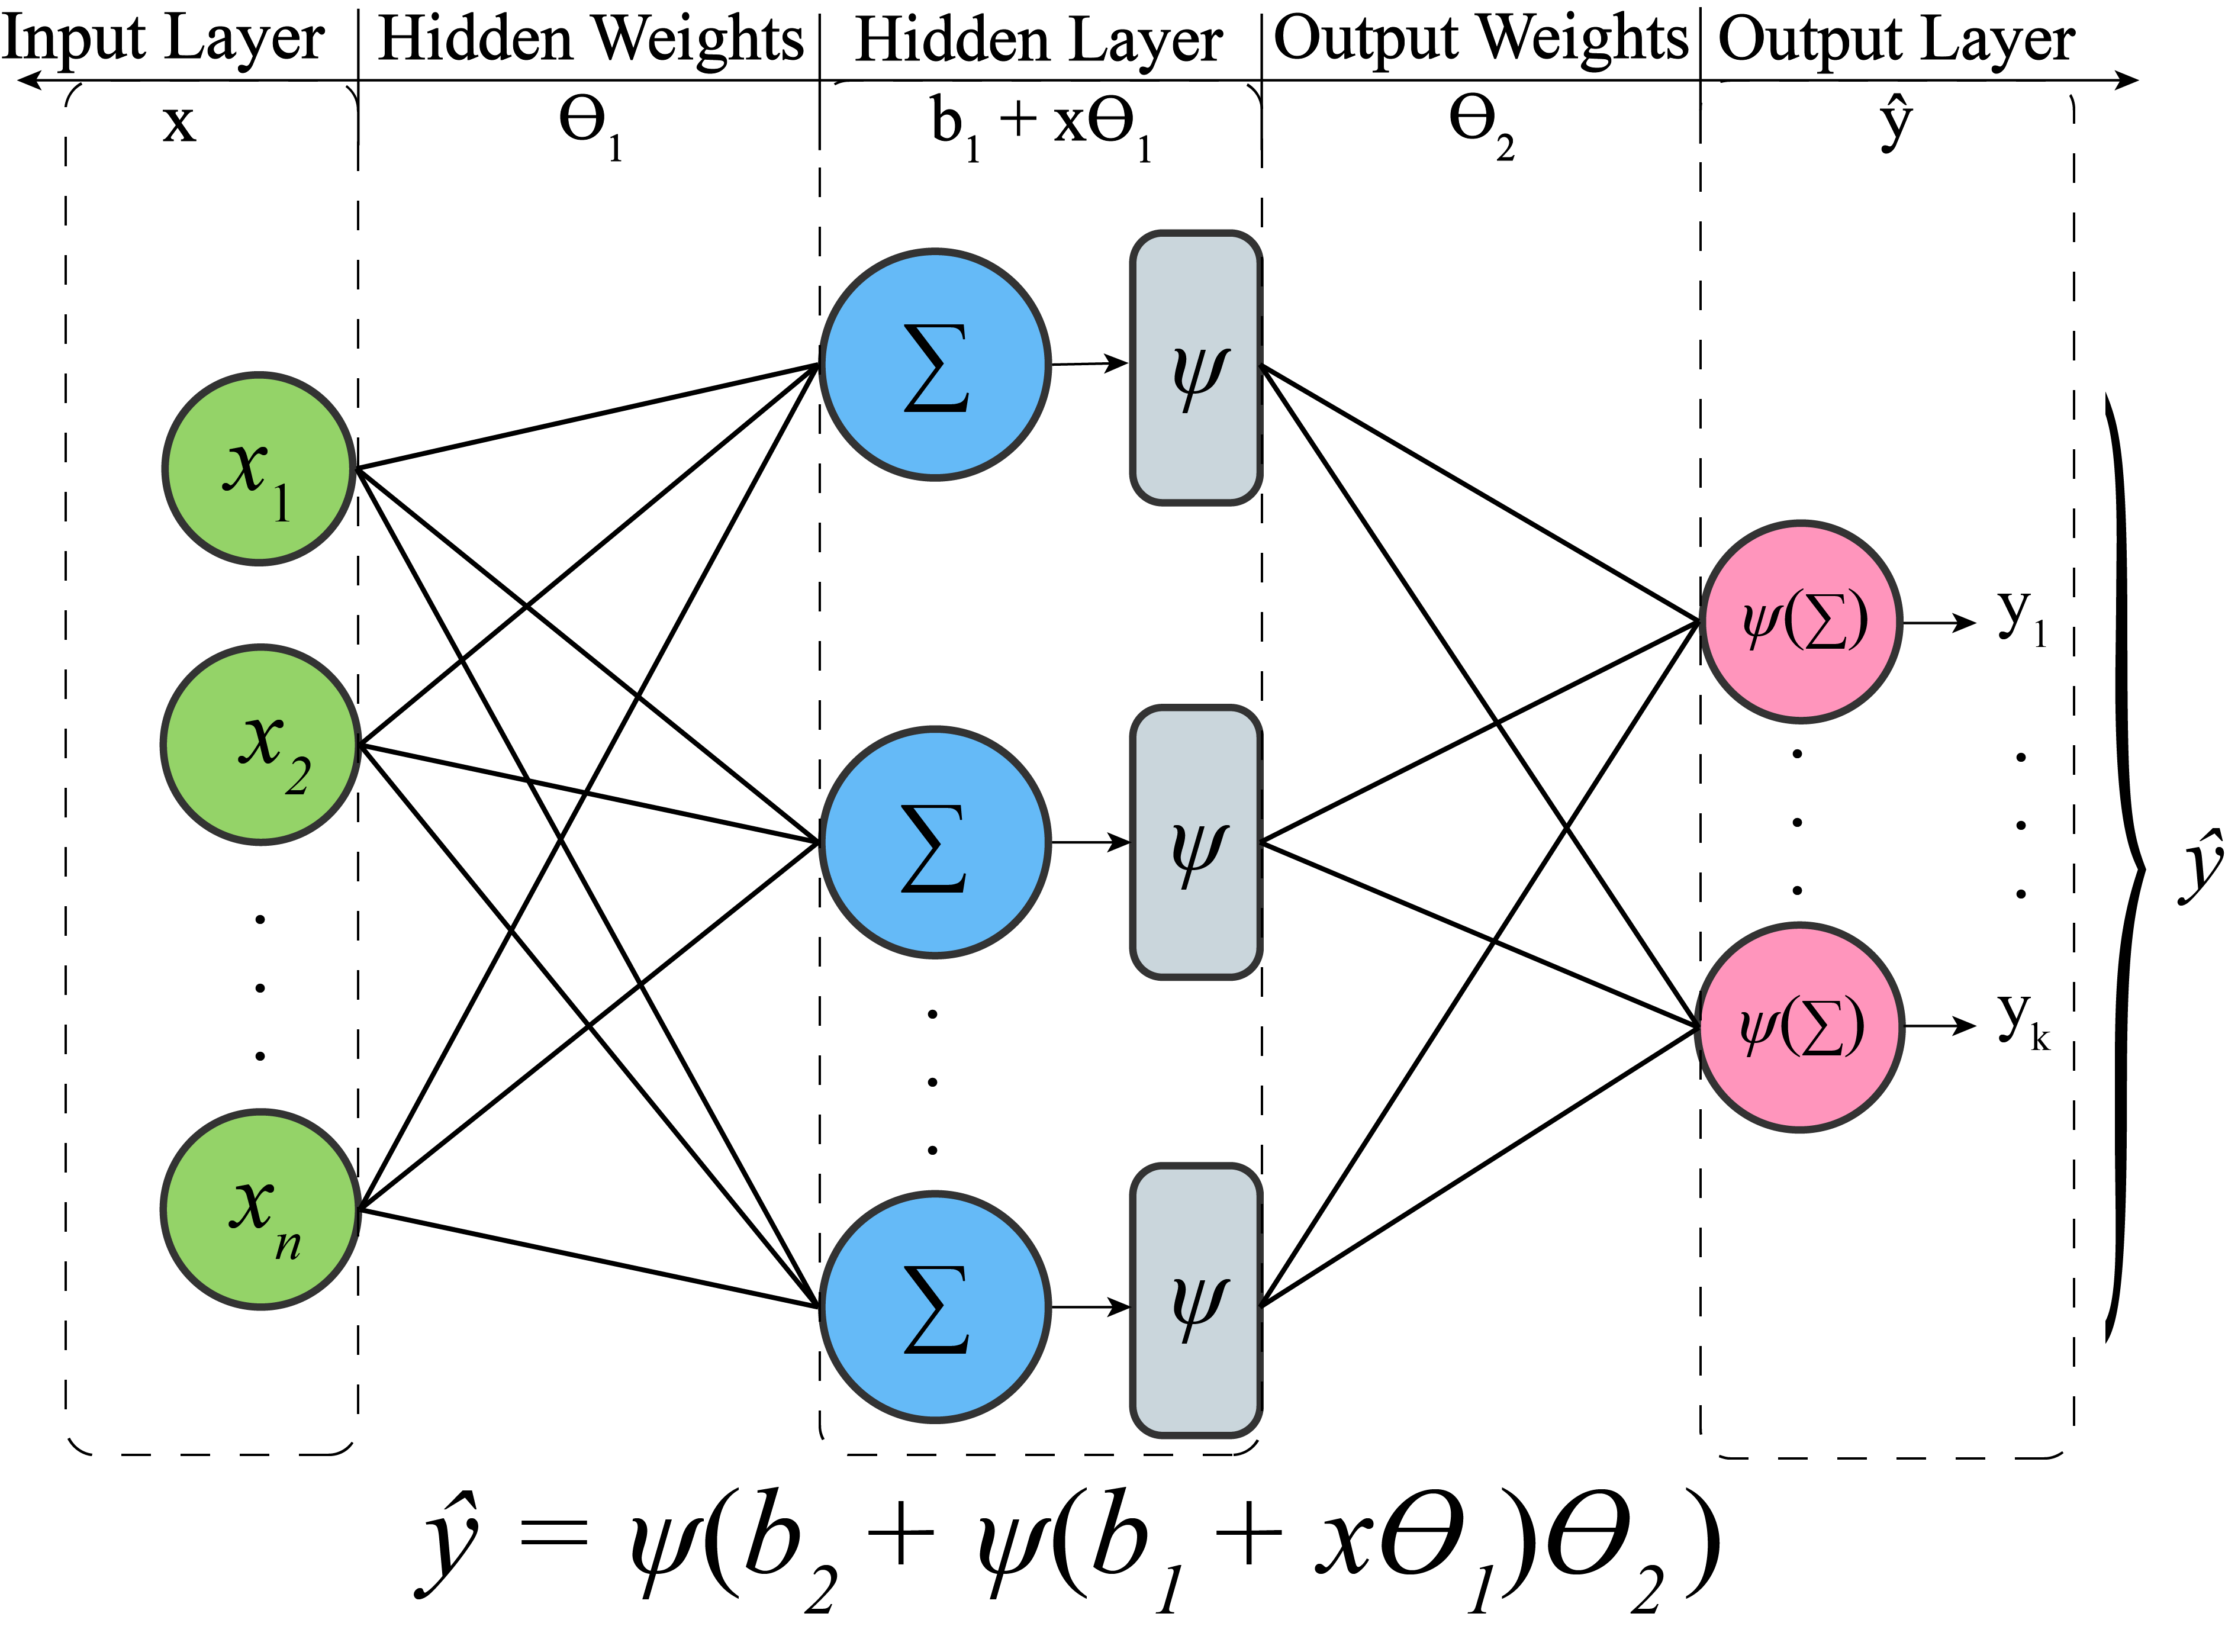
\includegraphics[height = 6cm, width=0.5\textwidth]{img/mlp.png}\label{fig:mlp}}
        %\caption{Feed Forward Multilayer Perceptron}
    \hfill
        \sidesubfloat[]{\includegraphics[height = 6cm, width=0.4\textwidth]{img/actfunc.png}\label{fig:actfunc}}
        %\caption{Common Activation Functions, $\psi$}
        
    \caption{a) Structure of a feed forward MLP with three layers. b) The output for Logistic, Tanh and ReLU activation functions for input value range [-4,4].}\label{fig:mlp_actfunc}
\end{figure}
% Change the italics brackets to regular 
% Add activation function to hidden layer 
%Define supervised classification

A nonlinear activation function $\psi$ allows the compositional output function $ \hat{y}$ to map inputs non-linearly to outputs. Deeper MLPs will contain many more hidden layers then displayed in Fig. \ref{fig:mlp} and a neural network with $n$ layers can be defined recursively as:
\begin{equation}
        \hat{y} = \psi(\theta_{n}(\psi(\theta_{n-1}(\psi(\theta_{n-2}(\ldots \psi(\theta_{1} x + b_{1}) \ldots)) + b_{n-2})) + b_{n-1}) + b_{n}),
\end{equation}

\noindent
,where the structure of $\hat{y}$ depends on the desired task (e.g nonlinear regression or classification). For regression problems, $\hat{y}$ is a real value, and for classification problems, $\hat{y}$ is a $k$ dimensional vector of real values. So although it is generally advantageous for hidden units to have nonlinear activation functions, the choice of activation functions for output layers will largely depend on the desired task. For nonlinear regression, a linear activation function is generally adequate. However, in classification problems, it can be useful to view the $k$ dimensional output vector $\hat{y} = (y_1,y_2,..., y_k)$ as providing the probabilities a given input example resides in each respective class. This produces a probability distribution over the $k$ classes, where entries fall between $(0,1)$, and the sum of the vector $\hat{y}$ is one. This behaviour can be accomplished by the softmax function:
\begin{equation}
       \mathrm{softmax}(z) = \frac{e^{z_j}}{\sum_{i=1}^{k}e^{z_i}} \;\;\; \mbox{for} \;\;\; j = \{1 \ldots k\},
\end{equation}

\noindent
where softmax$(z)$ represents the categorical distribution of arbitrary $k$ dimensional vector $z$. Furthermore, with a formally defined arbitrary output function $\hat{y}$, the next step requires the artificial neural network to learn weights and biases in order to produce desired outputs given input data.

\subsubsection{The Cost Function}
Training an artificial neural network relies on determining the network parameters that minimize the error between outputs $\hat{y}$ and true values $y$. This entails producing a model function, that given inputs, can produce the output to the closest degree. In machine learning, the notion of a good model is explicitly defined using some cost function $J(\hat{y},y;\Theta)$, where $\Theta = \{\theta, b\}$ is the set of all network weights and biases. The cost function keeps track of the model's prediction error. Finding better models equates to finding better network parameters that minimizes the cost function. For nonlinear regression, a commonly used measure of cost is simply the mean squared error between the output of the neural network and the true values:
\begin{equation} \label{eq:mse} 
    J(\hat{y},y;\Theta) = \sum_{i=1}^{m}(y_i - \hat{y_i})^{2}
\end{equation}

For classification problems, it is often beneficial to represent categorical true labels $y$ as binary vectors. This is referred to as one hot encoding, where the $i$th position of class $i$ is one, and every other term is zero. For example, in a five class problem, a class of three would be coded as $y = [0,0,1,0,0]$. In this way, the error must be calculated for each potential class $k$ over all examples in the sample set. Accordingly, the most commonly used cost function for classification problems is the cross entropy loss:
\begin{equation} \label{eq:softmax}
    J(\hat{y}, y; \Theta) = - \frac{1}{m}\sum_{i = 1}^{m}\sum_{j = 1}^{k} \lbrack y_{i,j} \log(\hat{y_{i,j}}) + (1 - y_{i,j})\log(1 - \hat{y_{i,j}}) \rbrack
\end{equation}

In the computation of cross-entropy loss, $k$ error terms are generated for every training example. The cross-entropy loss represents the log probability of classes given the model - that is, maximizing the likely hood of a training example belonging to a specific class is equivalent to minimizing the cross entropy loss between $\hat{y}$ and $y$. 

\subsubsection{The Optimization Algorithm}
The cost, $J(\hat{y}, y; \Theta)$, is conveniently a function of the training examples and model parameters $\Theta$. In order to effectively minimize the cost function, it is useful to observe how the cost changes with respect to weights $\theta$. Formally, this is expressed with the partial derivative $\frac{\partial J}{\partial \theta}$. With this expression, we can search for weights in the direction that cost $J$ decreases. This technique, called gradient descent, minimize cost by iteratively updating $\theta$ in the opposite direction of the gradient:

\begin{equation}\label{eq:update}
    \theta_j = \theta_j - \alpha \frac{\partial}{\partial \theta_j} J(\hat{y},y;\Theta) \;\;\; \mbox{for} \;\;\; j = \{1,\ldots,n\},
\end{equation}

\noindent
where $\alpha$, the learning rate, controls the size of steps made in the direction of the negative gradient. Furthermore, in order to compute the gradients of the cost with respect to model weights, an algorithm called backpropagation is commonly used. The cost function, as one large nested composite function, contains all of the computations in the neural network. With this, the backpropagation algorithm cleverly applies the chain rule of calculus to recursively compute the gradients of each weight, as shown in Fig. \ref{fig:backprop}. 

%with respect to the outputs so weights can be updated incrementally using gradient descent. 

\begin{figure}[htb]
    \centering
    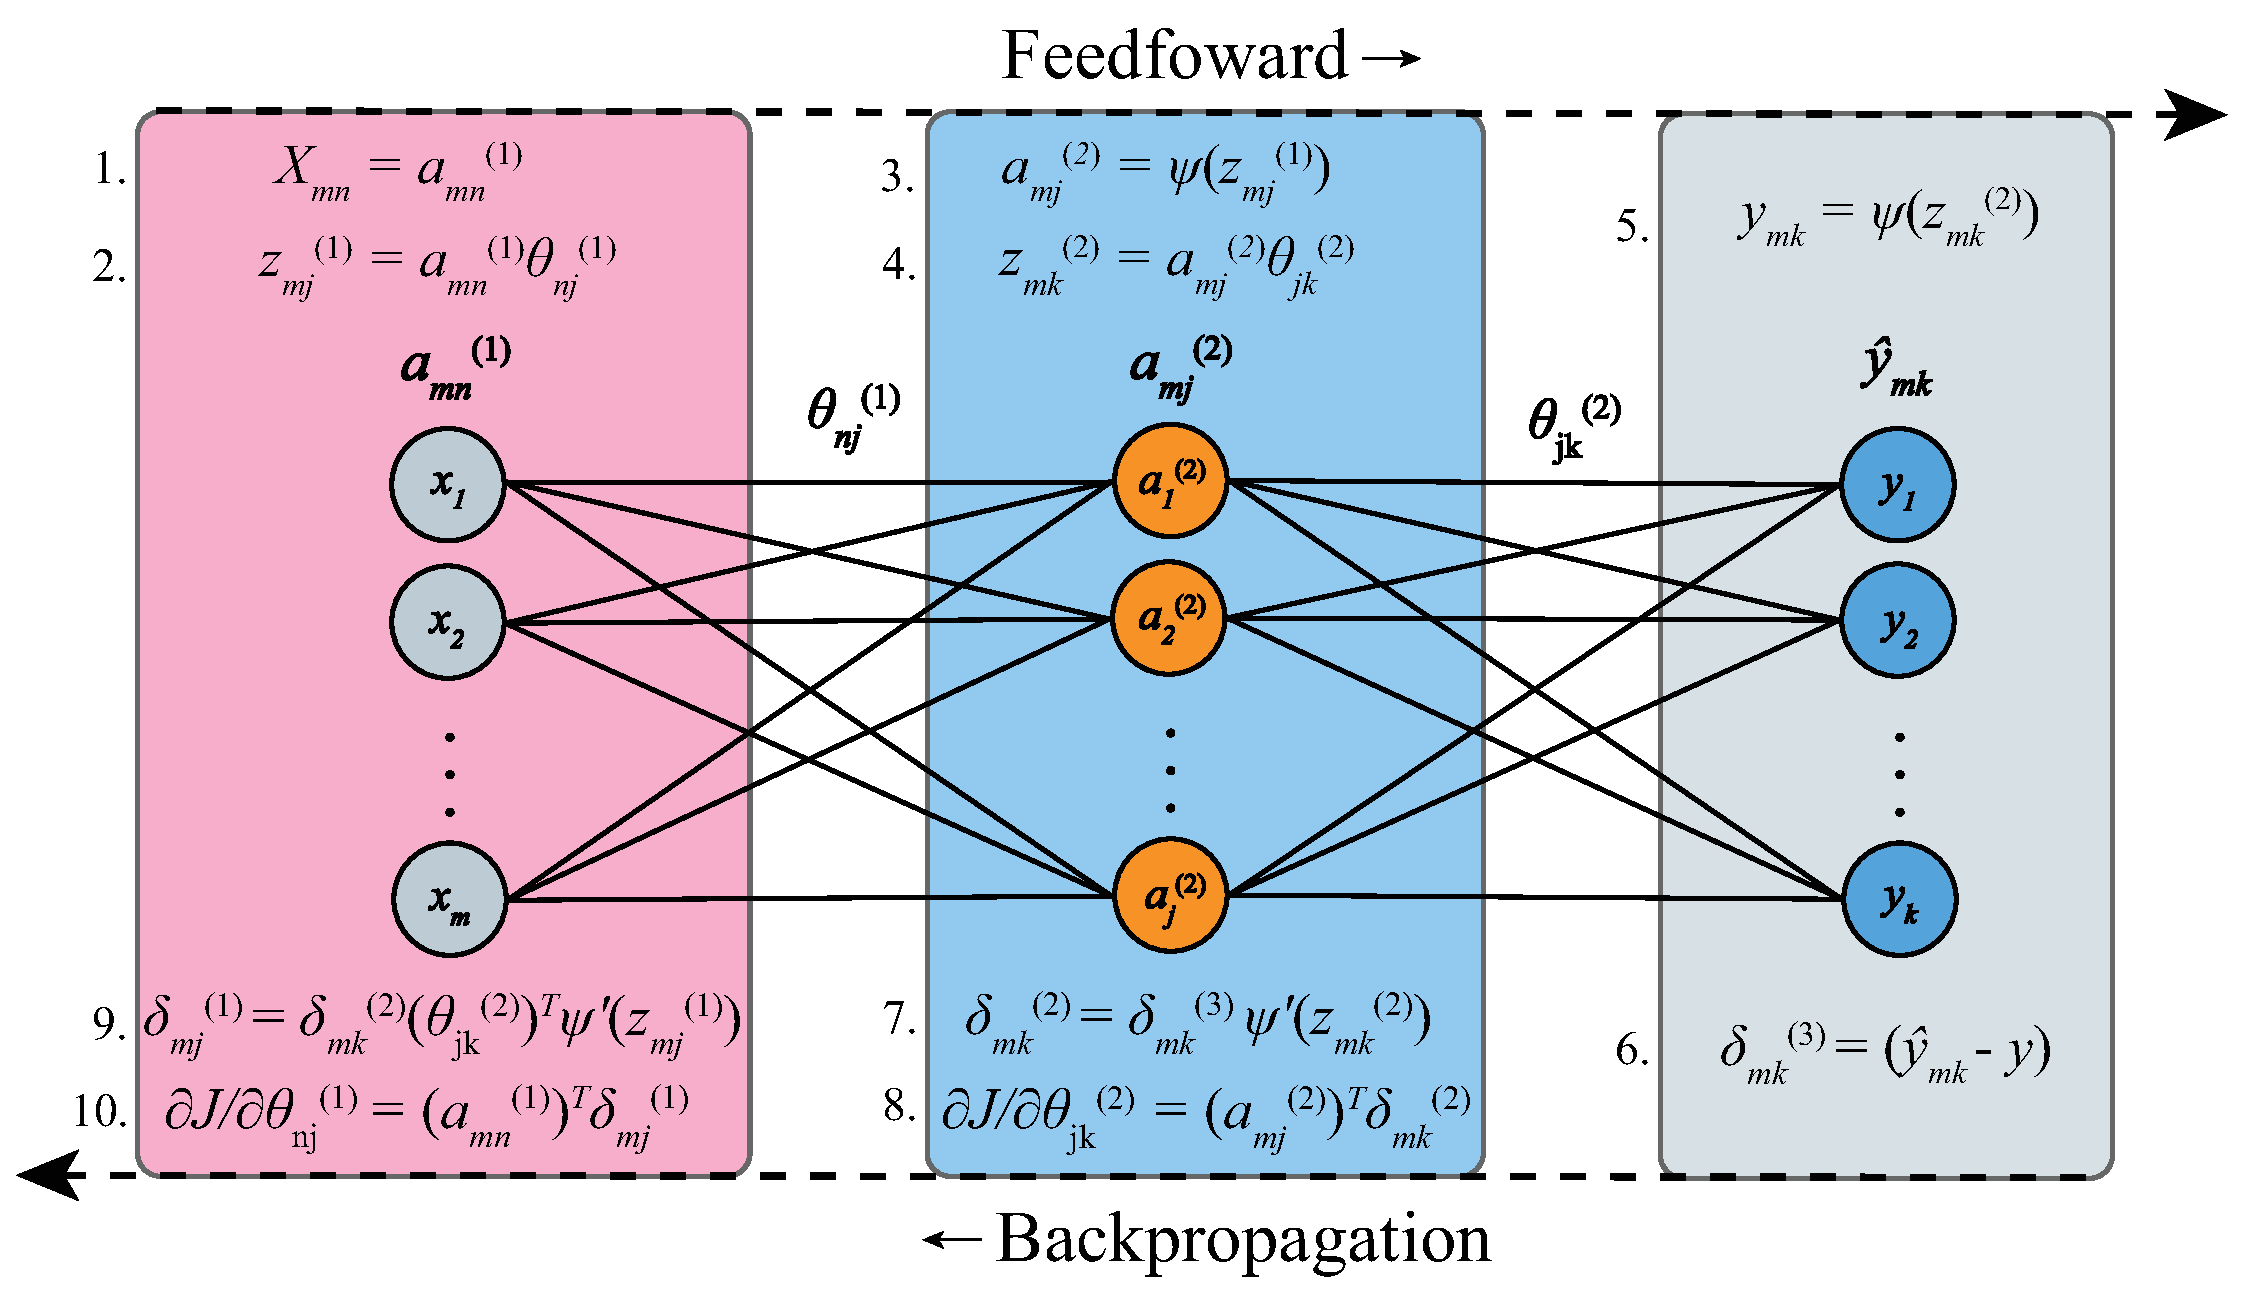
\includegraphics[width=\textwidth]{img/backprop.eps}
    \caption{Feedforward and Backpropagation Schematic.}
    \label{fig:backprop}
\end{figure}

Fig. \ref{fig:backprop} illustrates the mechanism of a feedforward multilayer perceptron with an input layer $X_{mn}$, a hidden layer $a_{mj}^{(2)}$, and an output layer $\hat{y}_{mk}$. The input layer, considered the first activation $a_{mn}^{(1)}$, is used to form the first linear combination $z_{mf}^{(1)}$. In the hidden layer, a nonlinear activation function $\psiup(z_{mj}^{(1)})$ is used to produce the hidden activations $a_{mj}^{(2)}$. In deeper networks, the preceding layers outputs are continually utilized in a series of linear combinations, following by nonlinear activation functions until the output layer is reached. At this point, the model predictions are compared to the true values using cost function $J(\hat{y}_{mk})$. In order to train the neural network, or minimize the cost function, the gradient of the cost function is computed to determine the direction in the parameter space required to lower network error. The gradient of the cost function is computed efficiently propagating the error back through the network using the derivate chain rule. In Fig. \ref{fig:backprop}, backpropagation begins with the output \textit{backpropagation-error} $\delta_{mk}^{(3)} = (\hat{y_{mk}} - y_{mk})$ shown in step 10. \textit{Backpropagation-error} is the layer specific approximation error, and the hidden and input layer \textit{backpropagation-errors} are represented as $\delta_{mk}^{(2)}$ and $\delta_{mf}^{(1)}$, respectively. In Eq. \ref{eq:update}, we see that the partial derivative of the cost function with respect to each weight is required in order to compute a gradient update. In this example, the weights of the model are spread across two matrices, $\theta_{nf}^{(1)}$ and $\theta_{jk}^{(2)}$. Accordingly, we will calculate gradient matrices of the same dimension, $\partial J / \partial \theta_{nf}^{(1)}$ and $\partial J / \partial \theta_{jk}^{(2)}$, to store the gradient of the cost function with respect to each weight in the model. Starting with $\partial J / \partial \theta_{jk}^{(2)}$, we get the following expression using squared error as the cost function:

\begin{equation*}
    \frac{\partial J}{\partial \theta_{jk}^{(2)}} =  \frac{\partial \frac{1}{2}\sum (y_{mk} - \hat{y}_{mk})^{2}}{\partial \theta_{jk}^{(2)}}
\end{equation*}

\noindent
If we remove the summation from this expression we can compute the gradient for a single example. Evaluating the resultant derivative produces:

\begin{equation*}
    \frac{\partial J}{\partial \theta_{jk}^{(2)}} =  -(y_{mk} - \hat{y}_{mk})\frac{\partial \hat{y}_{mk}}{\partial \theta_{jk}^{(2)}}\\
\end{equation*}

\noindent
From step 5 on Fig. \ref{fig:backprop}, we see that $\hat{y}_{mk} = \psiup(z_{mk}^{(2)})$. Accordingly, we can now apply the chain rule to further evaluate the expression: 

\begin{equation*}
    \frac{\partial J}{\partial \theta_{jk}^{(2)}} =  -(y_{mk} - \hat{y}_{mk}) \frac{\partial \hat{y}_{mk}}{\partial z_{mk}^{(2)}} \frac{\partial z_{mk}^{(2)}}{\partial \theta_{jk}^{(2)}}\\
\end{equation*}

\noindent
We can now replace $\partial \hat{y}_{mk} / \partial z_{mk}^{(2)}$ with $z_{mk}^{(2)}$ evaluated by the derivative of the activation function, $\psiup'(z_{mk}^{(2)})$. As well, from step 4 on Fig. \ref{fig:backprop}, we see that $z_{mk} = a_{mj}^{(2)}\theta_{jk}^{(2)}$. The derivative of this linear relationship is simply the slope $a_{mj}^{(2)}$. We can now simplify our expression:

\begin{equation*}
    \frac{\partial J}{\partial \theta_{jk}^{(2)}} =  -(y_{mk} - \hat{y}_{mk}) \psiup'(z_{mk}^{(2)}) a_{mj}^{(2)}
\end{equation*}

\noindent
The hidden layer \textit{backpropagation-error} is given by $\delta_{mk}^{(2)} = -(y_{mk} - \hat{y}_{mk})\psiup'(z_{mk}^{(2)})$. Notice that if we transpose the activity matrix $a_{mj}^{(2)}$, we can perform matrix multiplication with $a_{mj}^{(2)}$ and $\delta_{mk}^{(2)}$ to sum across all examples. This effectively takes care of the earlier omission of the summation, so that the gradient can be calculated efficiently as shown in step 8 on Fig. \ref{fig:backprop}. The simplified expressions becomes:

\begin{equation*}
    \frac{\partial J}{\partial \theta_{jk}^{(2)}} =  (a_{mj}^{2})^{T}\delta_{mk}^{(2)}
\end{equation*}

\noindent
The derivation for $\partial J / \partial \theta_{nj}^{(1)}$ begins the same way as described above, but diverges when the chain rule is used to expand $\partial z_{mk}^{(2)}/\partial \theta_{nj}^{(1)}$:
 
\begin{equation*}
\begin{split}
\frac{\partial J}{\partial \theta_{nj}^{(1)}} & = \delta_{mk}^{(2)} \; \frac{\partial z_{mk}^{(2)}}{\partial \theta_{nj}^{(1)}} \\
 & = \delta_{mk}^{(2)} \; \frac{\partial z_{mk}^{(2)}}{\partial a_{mj}^{(2)}} \; \frac{\partial a_{mj}^{(2)}}{\partial \theta_{nj}^{(1)}}\\
& = \delta_{mk}^{(2)} \; (\theta_{jk}^{(2)})^{T} \; \frac{\partial a_{mj}^{(2)}}{\partial \theta_{nj}^{(1)}}\\
& = \delta_{mk}^{(2)} \; (\theta_{jk}^{(2)})^{T} \; \frac{\partial a_{mj}^{(2)}}{\partial z_{mf}^{(1)}} \; \frac{\partial z_{mf}^{(1)}}{\partial \theta_{nj}^{(1)}}\\
& = \delta_{mk}^{(2)} \; (\theta_{jk}^{(2)})^{T} \; \psiup'(z_{mf}^{(1)}) \; \frac{\partial z_{mf}^{(1)}}{\partial \theta_{nj}^{(1)}}\\
& = (a_{mn}^{(1)})^{T} \; \delta_{mk}^{(2)} \; (\theta_{jk}^{(2)})^{T} \; \psiup'(z_{mf}^{(1)})\\
& = (a_{mn}^{(1)})^{T} \; \delta_{mj}^{(1)}
\end{split}
\end{equation*}

\noindent
The simplified expression for both gradients are closely related. We see that the gradients depend on the layer activity and the \textit{backpropagation-error}. In turn, the calculations for \textit{backpropagation-error} are dependent on the error terms in the next layer. Thus, computation of error proceeds backwards from the output layer towards the input layer. This is where backpropagation, or backwards propagation of errors, gets its name. The error $\delta^{\ell}$ at layer $\ell$ is dependent on the errors $\delta^{\ell+1}$ at the next layer $\ell + 1$. 

%In Figure \ref{fig:actfunc}, we see that the tanh and logistic functions have sigmoidal shapes, mapping all inputs between $(-1,1)$ and $(0,1)$, respectively. In the output layer, this kind of behaviour makes them useful for classification problems. Though for nonlinear regression, a linear output activation would be beneficial. Accordingly, the choice of activation functions will largely depend on the desired task, but it is generally desired for the hidden units to have nonlinear activation functions. Deeper MLPs will contain many more hidden layers then displayed in Figure \ref{fig:mlp}, 

%%The cost function, as one large nested composite function, contains all of the computations in the neural network. 

\section{Deep Learning} \label{sec:deeplearning}

\subsection{Deep Neural Networks}

%Explain what deep learning is, why it is used (representation learning)

Deep learning is a subset of machine learning based on artificial neural networks. Deep learning employs architectures such a deep neural networks (DNN) that typically have multiple layers between the input and the output layers. DNNs learn hierarchical representations of the data through the layers of the network in order to map complex relationships between the input and the desired outputs. Recently, these networks have made state-of-the-art breakthroughs in fields such as natural language processing, computer vision, and speech recognition.

DNNs are especially useful for learning intermediate representations of input data. The representations are formed with the composition of non-linear transformations through multiple layers in the network. The output of each layer forms a hierarchy of distributed representations that have an increasing level of abstraction as an input flows through the network. The performance of a DNN depends largely on the representations it learns to output. This is because the distribution of the input data is generated by a combination of underlying features and a model that learns to compactly represent the features can generalize for more variation without requiring as many examples. In cases where the transformation results in data compression the learning task equates to developing output representations that map to the naturally occurring input data distribution but in a low dimensional manifold.

\subsection{Autoencoders}

Autoencoders represent a family of unsupervised artificial neural networks that learn latent data codings for input data. Here, training examples are utilized without labels, and autoencoders are trained to generate outputs identical to the inputs. The role of an autoencoder is split into two tasks, encoding and decoding. The process of encoding maps the input to lower dimension features, and decoding maps the encoded data back into the original space. The mapping of an input layer produced by function, $g_{\theta}(\cdot)$, can be expressed as:
 
\begin{equation}
z = g_{\theta}(x) = \psi(\theta x + b)
\end{equation}

This latent layer, of potentially reduced dimensionality, can then be decoded back to the original space with function $f_{\theta^{T}}(\cdot)$:

\begin{equation}
x' = f_{\theta^{T}}(z) =  f_{\theta^{T}}(g_{\theta}(x)) = (\theta^{T}z + b)
\end{equation}

Where $x'$ is the reconstructed input data, and $\theta^{T}$ is the transpose of weights used for encoding. Furthermore, to train the model, the reconstructed output is compared to the original input using the mean squared error to calculate reconstruction error:

\begin{equation}
J(x'_{i},x_{i};\Theta) = \frac{1}{2m}{\sum^{m}_{i=1}} ||x_i - x'_i||^2
\end{equation}

Where $\Theta = \{\theta, b_\theta,\theta^{T}, b_{\theta^{T}}\}$ is the set of network parameters used for encoding and decoding operations. 

\subsubsection{Denoising Autoencoders}
Training an autoencoder with partially corrupted data while comparing the reconstruction to the original input is a commonly used technique to increase the robustness of an autoencoder. This modification produces a variant of the basic autoencoder called a denoising autoencoder. By adding corruption to the input data, $\tilde{x}_{i} \sim \mu_{D}(\tilde{x}_{i}|x_{i})$, the autoencoder must learn parameters that can overcome stochastic noise. The operation $\mu_{D}$ defines the form of noise used to corrupt the input data in order to increase robustness, and the reconstruction error is calculated using cost $J(\tilde{x}'_{i},x_{i};\Theta)$. 

Furthermore, deeper frameworks of denoising autoencoders, called stacked denoising autoencoders (SDAEs), are employed to increase the number of latent abstractions. SDAEs are composed of multiple layers of incrementally stacked denoising autoencoders that are trained one layer at a time \cite{vincent2010stacked}. In this way, once the $k$th hidden layer is trained, layer $k+1$ can be trained using the $k$th layer as the input data.

% Add figures for stacked denoising autoencoder

\section{Improving Machine Learning Models}

\subsection{Regularization}
%Talk about overfitting
%Regularization

A key aspect of producing a good machine learning model is to avoid overfitting the training data. The problem of overfitting arises when the model variables and parameters aggressively captures both the underlying pattern and stochastic noise of the training data. The model is learning information that does not represent the true properties of the underlying relationship when it captures too much random noise. In this case, the model will perform well on the test set, but will likely have a poor prediction and generalization power on examples it has never seen before. 

This problem gets worst as the model complexity increases, and the model variables and paramaters have the flexibility to increasingly capture background noise. A way to avoid overfitting is by using cross validation. Cross validation is beneficial because the model variables and parameters are decided by estimating the error of the model over a subset of the data the model has not observed. In $k$-fold cross validation, this is performed by dividing the data into $k$ subsets. Then each of the $k$ subsets are used as a validation set, and the other $k-1$ subsets are combined as the training set. Accordingly, the error estimation gets averaged over the $k$ trials to compute the total effectiveness of the model.

Furthermore, another commonly used way to avoid overfitting is through model regularization. Regularization is a form of regression that applies a constraint to the model complexity. Ridge regression involves penalizing the cost function during the training procedure by adding a multiple of the squared magnitude of the model coefficients. Accordingly, ridge regression employs weighted L2 regularization producing the following loss equation:

\begin{equation} \label{eq:l2reg}
    \mathrm{Loss} = J(\hat{y},y;\Theta) + \frac{\lambda}{2m} \sum_{j=1}^{m} \sum_{k=1}^{p} \Theta_{j,k}^{2} \;\;,
\end{equation}

\noindent
where m is the number of training examples, p is the number of model weights, and $\lambda$ is the regularization parameter. Here, $\lambda$ decides how much the model flexibility should be penalized. When $\lambda = 0$, the penalty term is ignored, and the trained model is susectible to overfitting. However, as $\lambda \rightarrow \infty$, the model weights are increasingly penalized and will approach zero. This will result in under-fitting, where the model losses the ability to fit the data entirely. Therefore, selecting a good regularization parameter is essential for optimizing the performance of the machine learning model. 


\subsection{Model Averaging}
%Model Averaging - dropout and maxout model

The dropout technique is a relatively simple way to regularize a neural network using the concept of model averaging. Dropout entails randomly setting a fraction of the neurons in the network to zero during forward propagation. At each training step, a neuron is either kept with a probability of $p$, or \textit{dropped out} with probability $1-p$ to produce a network of reduced size. During backpropagation, the weights of dropped out neurons will not be updated. Accordingly, dropout is training a subsample of the whole neural network on every training iteration. In this way, dropout can be seen as an ensemble of randomly sampled models that share parameters. As well, dropout is a useful technique for addressing co-adapting behaviour in machine learning models. Co-adaptation occurs when neurons learn to fix the mistakes of other neurons in a fully connected neural network. This is a problem because co-adapted neurons tend to result in overfitting because they do not generalize well to new data. With dropout, neurons are forced to learn more robust features that are independent to the other neurons. 

\begin{figure}[htb]
    \centering
        \sidesubfloat[]{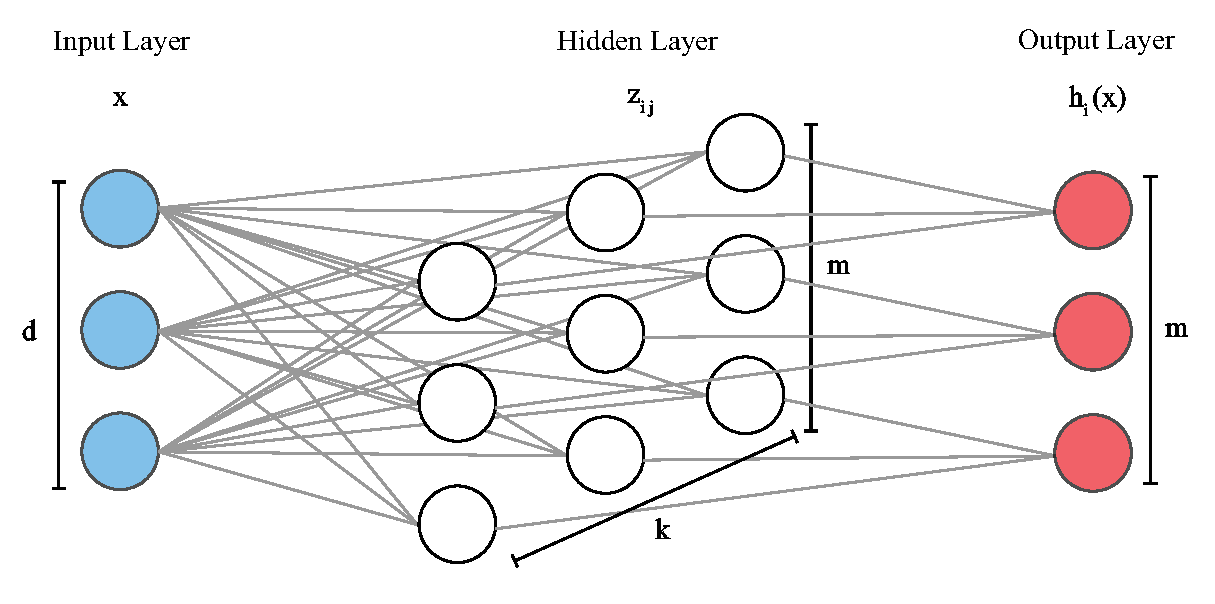
\includegraphics[width=0.7\textwidth]{img/maxout1.eps}\label{fig:maxout_a}}
        %\caption{Feed Forward Multilayer Perceptron}
    \hfill
        \sidesubfloat[]{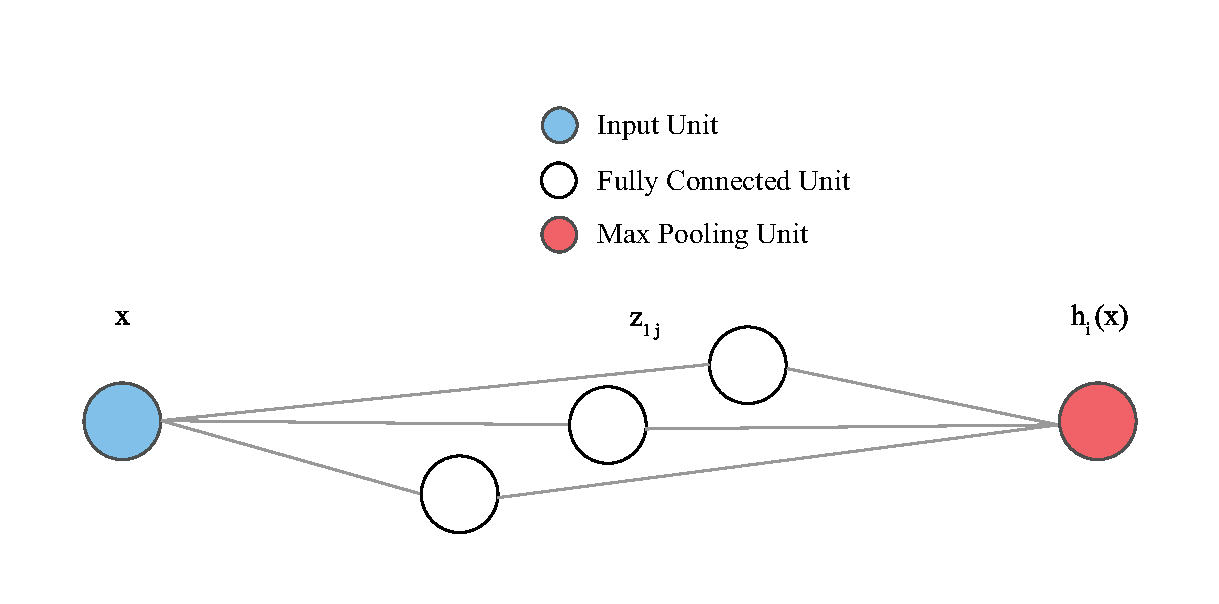
\includegraphics[width=0.7\textwidth]{img/maxout2.eps}\label{fig:maxout_b}}
        %\caption{Common Activation Functions, $\psi$}
        
    \caption{a) Structure of a maxout neural network b) Maxout neural network with d = 1, m = 1, and k =3}\label{fig:maxout}
\end{figure}

Furthermore, an activation function called maxout was proposed to leverage the model averaging performed by dropout \cite{goodfellow2013maxout}. The maxout activation function was shown to improve approximate model averaging in deep models over non-linear activations such as the Tanh function \cite{goodfellow2013maxout}. Formally, the maxout activation function is defined as: 

\begin{equation} \label{eq:maxout}
    h_{i}(x) = \underset{j \in [1,k]}{\mathrm{max}}z_{i,j},
\end{equation}

\noindent
where $x \in \mathbb{R}^{n}$ is an input vector, $z_{i,j} = x^{T}W_{...ij}v + b_{ij}$ is output for the $j$-th linear transformation of the $i$-th hidden unit, and $W \in \mathbb{R}^{d \times m \times k}$ and $b \in \mathbb{R}^{m \times k}$ are learned parameters. In simple terms, maxout accepts an input of dimensionality $d$ and computes $k$ linear transformations and returns the largest unit for each of the $m$ linear feature extractors. The maxout activation function is applied by using a small differentiable sub-network as shown in Fig. \ref{fig:maxout}.

\begin{figure}[ht]
    \centering
    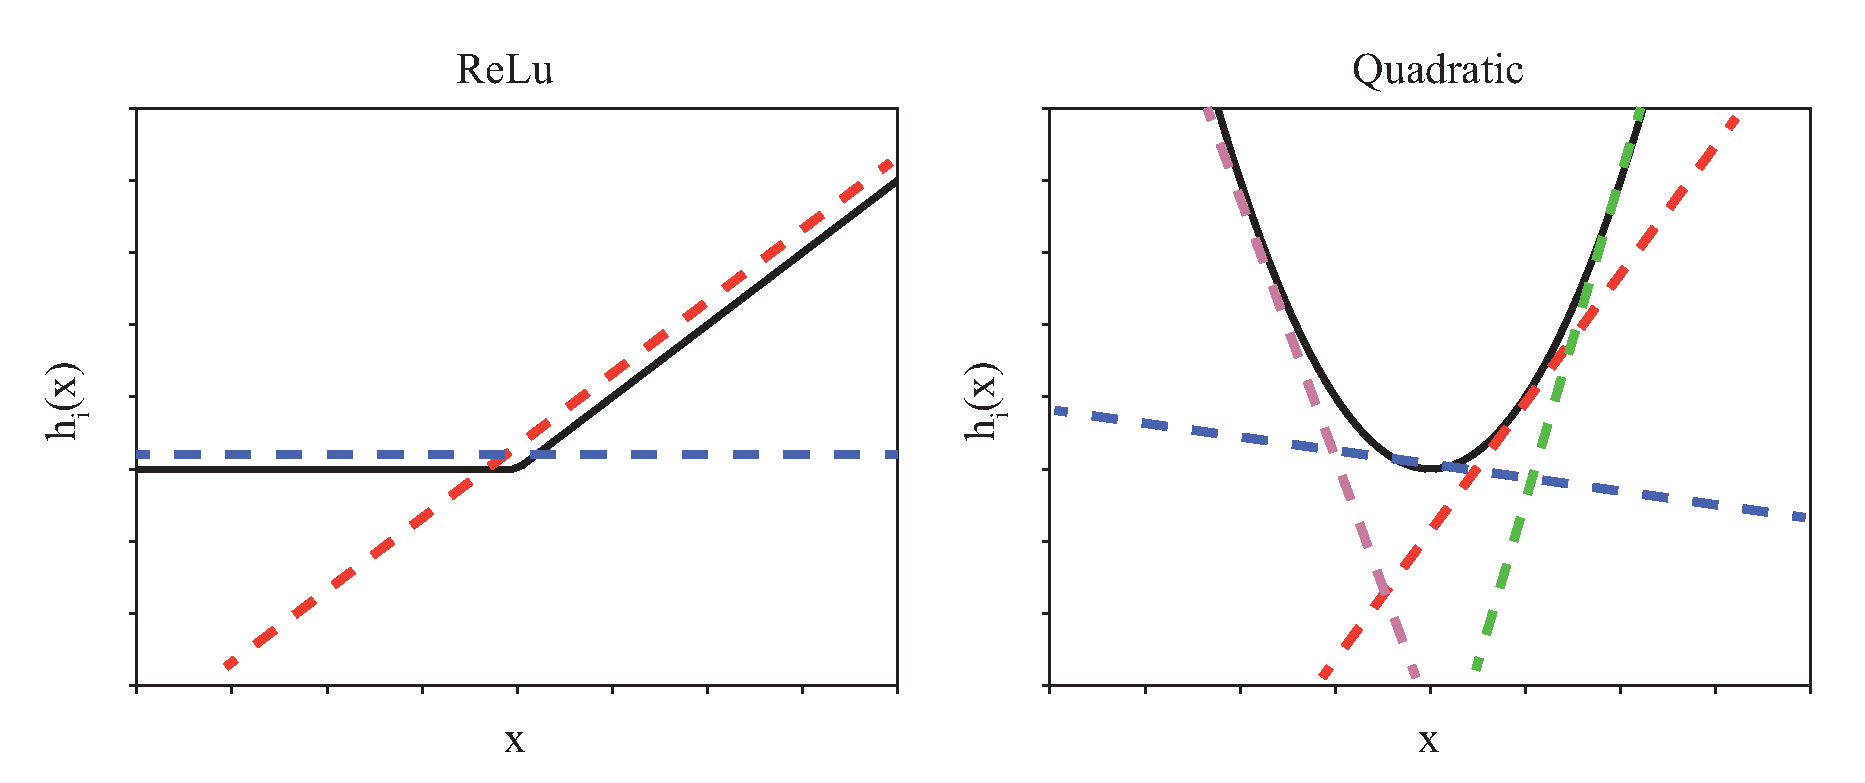
\includegraphics[width=0.7\textwidth]{img/max_func.eps}
    \caption{Maxout approximation of ReLu and quadratic activation functions.}
    \label{fig:maxout_func}
\end{figure}

In Fig. \ref{fig:maxout_a}, the hidden layer implements the weighted sum of all inputs. In Eq. \ref{eq:maxout}, this is represented by $z_{i,j} = x^{T}W_{...ij} + b_{ij}$. The three-dimensional tensor $W_{...ij}$, represents the weight vector for the unit in row $i$ and column $j$ of the fully connected units. The max pooling units simply take the maximum output from the neurons of each row. From Fig. \ref{fig:maxout_func}, we can see how the maxout activation function can approximate a ReLu and qaudratic activation function. In this way maxout can produce a piecewise linear approximation of an arbitrary convex function.
    \chapter{Related Work} \label{chap:relatedwork}

\section{Dimensionality Reduction}

\section{Information Fusion}

\subsection{Mixture of Experts}

\subsection{Gated Multimodal Units}
    \chapter{Deep Gated Multimodal Units} \label{chap:deepgmu}

In this chapter we propose a novel multimodal fusion approach to integrate information from multiple genomic sources. While most methods have solely relied on data fusion (early fusion) or decision level fusion (late fusion), our approach utilizes a series of cascading gated multimodal units to deeply connect the integration of data fusion and decision fusion.
%by a series of cascading layers

\section{Architecture}

The architecture of a dGMU first contains multiplicative gates designed to construct an intermediate representation of data from multiple modalities. The input modalities along with the intermediate representation are then fed to a decision network that fuses the predictions using an additional gate. These two processes can be subdivided into the function of a representation network and a decision network. In the representation network, the input modalities learn a latent representation of the combined input data. While the decision network makes predictions based on all representations and learns to decide how decisions influence the activation of the output unit. This structure is illustrated in Figure \ref{fig:dgmu}. 

\begin{figure}[h!]
    \centering
    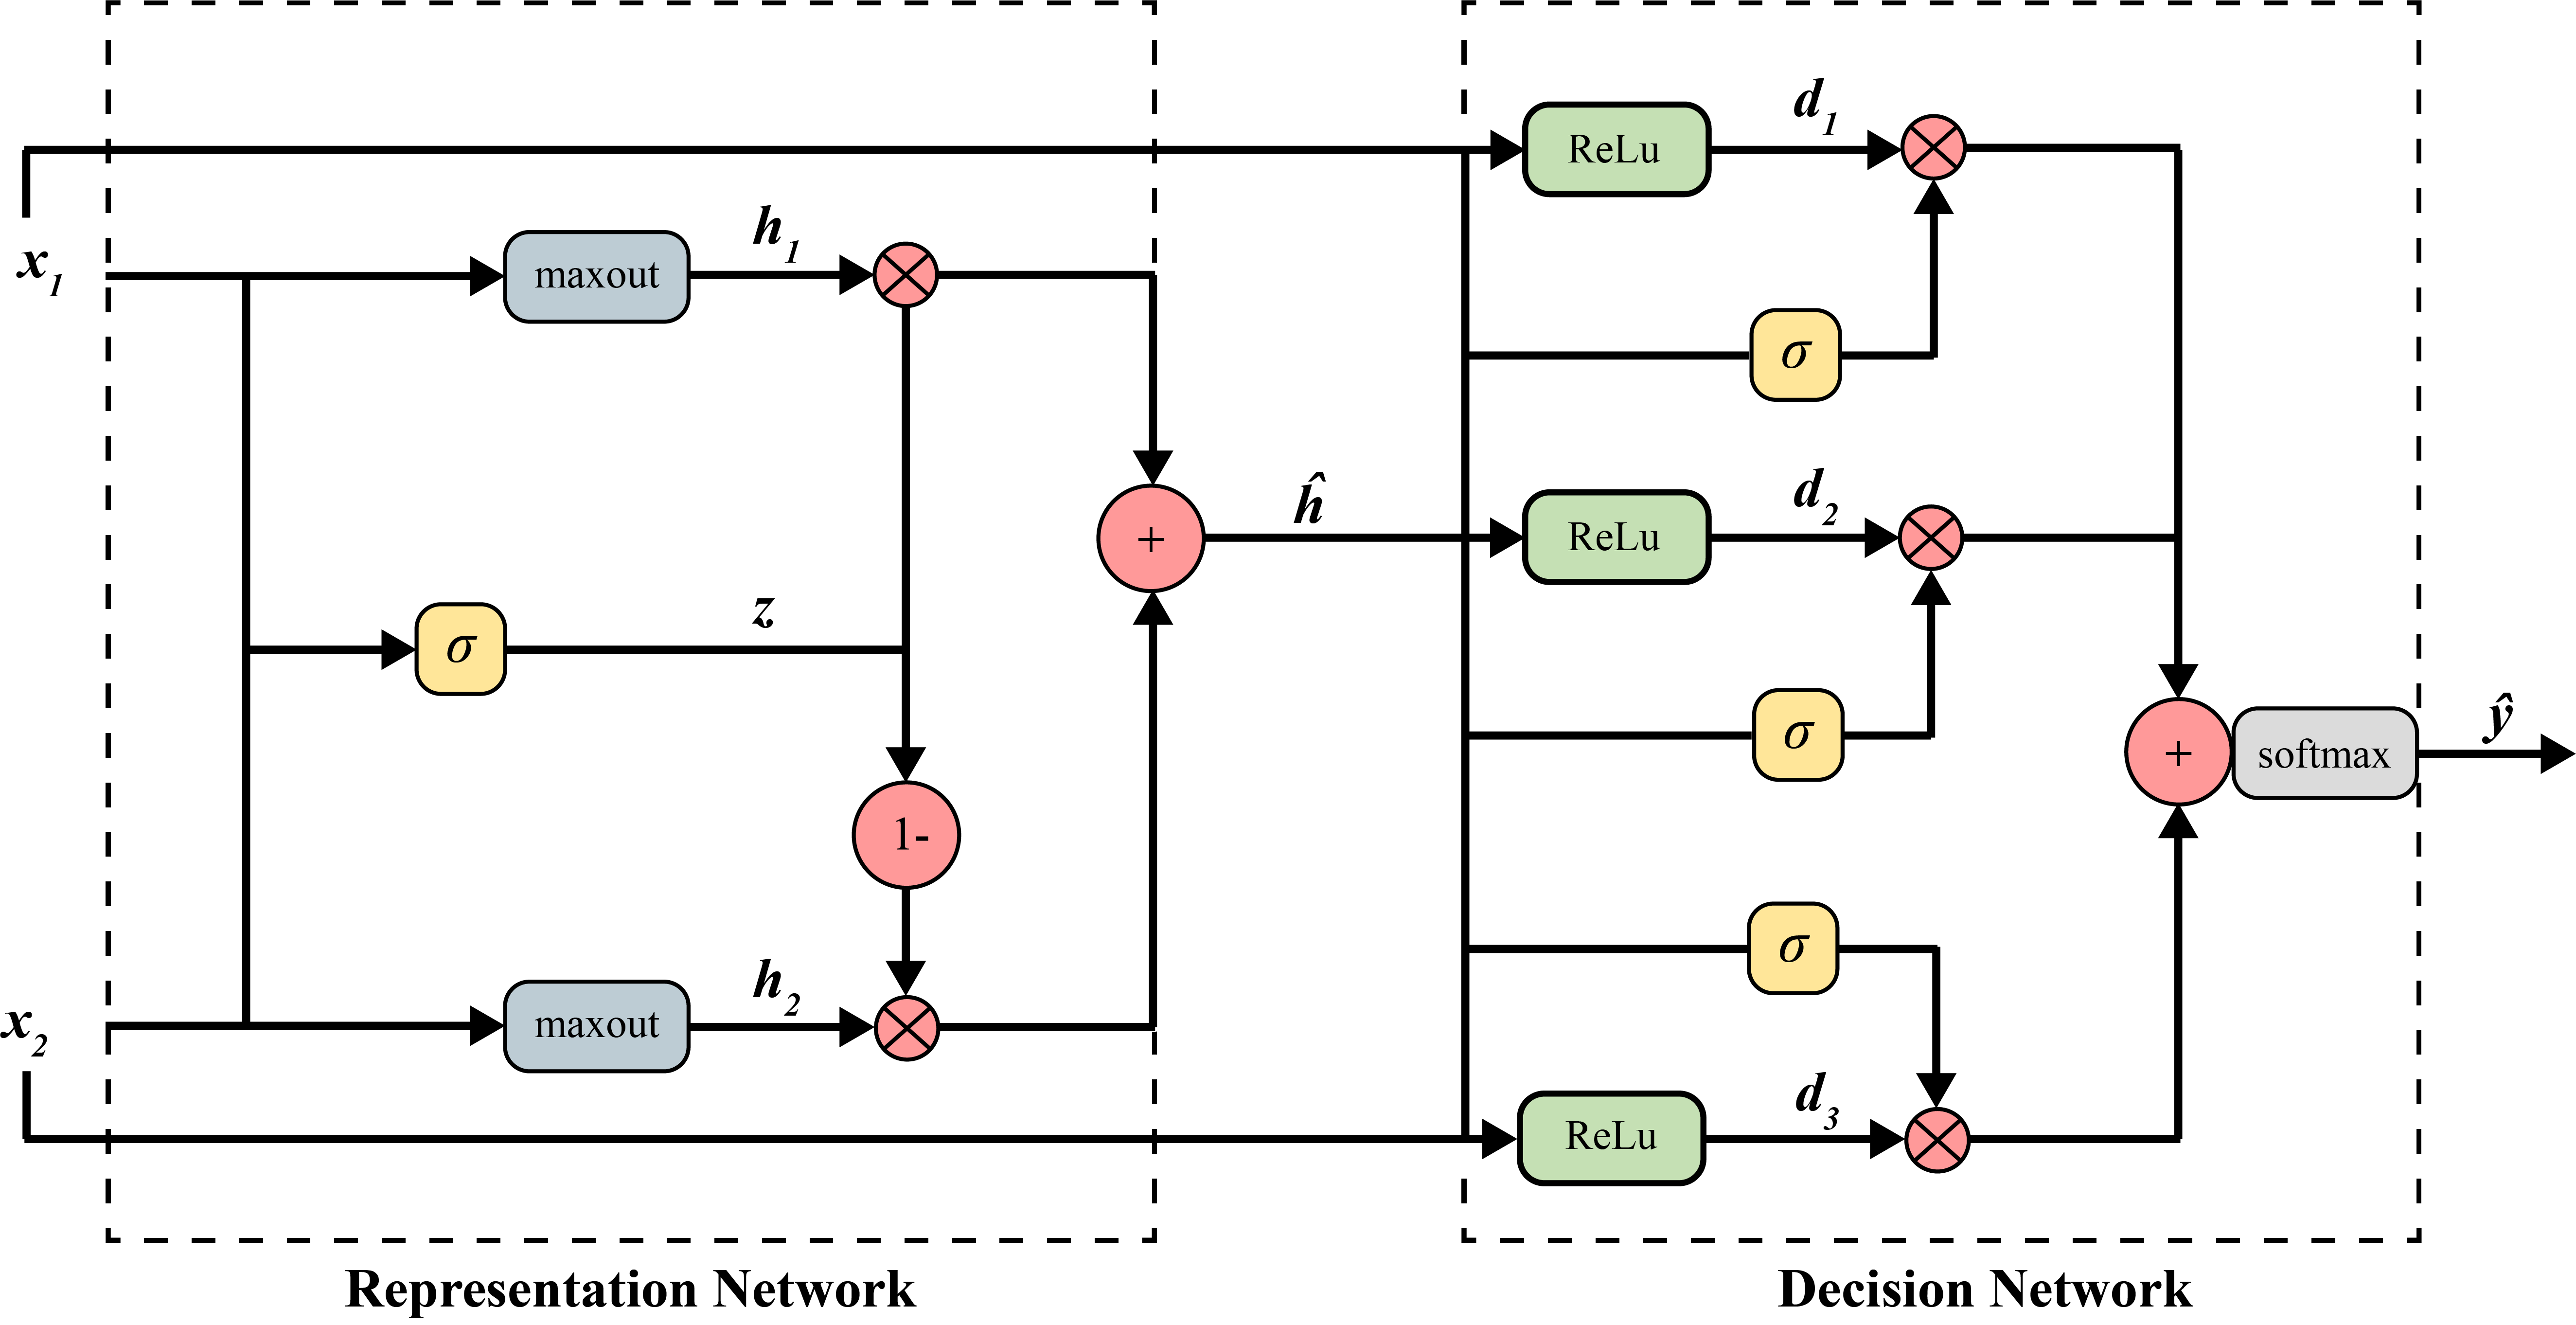
\includegraphics[width=\textwidth]{img/dGMU.png}
    \caption{Deep Gated Multimodal Unit.}
    \label{fig:dgmu}
\end{figure}

\noindent
The connection between the internal representation and decision networks are governed by the following equations:

\noindent
\textbf{Representation Network}
\begin{center}
    $h_1 = maxout(\theta_{h1} \cdot x_1)$\\
    $h_2 = maxout(\theta_{h2} \cdot x_2)$\\
    $z = \sigma(\theta_z \cdot [x_1,x_2])$\\
    $x_3(x_1,x_2;\Theta_R) = z * h_1 + (1-z)*h_2$\\
    %$\Theta_R = \left\{W_{h1},W_{h2},W_{x3}\right\}$\\
\end{center}

\noindent
Where latent space, $x_3(x_1,x_2;\Theta_R)$, depends on inputs $x_1$ and $x_2$, and $\Theta_R = \left\{\theta_{h1},\theta_{h2},\theta_{x3}\right\}$ is the set of network parameters used for encoding the latent space.

\noindent
\textbf{Decision Network}

\begin{center}
    $$
        \hat{y}(x_1,x_2,x_3;\Theta_D) = {\sum^{3}_{i=1}} ReLu(\theta_{di} \cdot x_i)\sigma(\theta_{di} \cdot [x_1,x_2,x_3])
    $$\\   
    %$\Theta_D = \left\{W_{d1},W_{d2},W_{d3},W_{g1},W_{g2},W_{g3}\right\}$\\
\end{center}

\noindent
Where the network output, $\hat{y}(x_1,x_2,x_3;\Theta_D)$, depends on inputs $x_1$, $x_2$, and $x_3$, and $\Theta_D = \left\{\theta_{d1},\theta_{d2},\theta_{d3},\theta_{g1},\theta_{g2},\theta_{g3}\right\}$ is the set of network parameters used across the untied gates in the decision network.

%Internal gating neuron
%representation network
%decision network

\section{Training}

%majahan

The dGMU model parameters were learned with batch stochastic gradient descent with ADAM optimization \cite{kingma2014adam}. The training complexity was reduced by using a supervised pre-training scheme on the decision network \cite{mahajan2018exploring}. This method is used to initialize the parameters of the decision network to ease the training of the larger model, reducing computation time and increasing model robustness \cite{clune2013evolutionary}. The complete network was optimized using supervised fine-tuning with the connected sub-networks. During the training process, overfitting was controlled using dropout and $L_2$ regularization. For classification problems the global loss is computed using the softmax cross entropy loss as seen in Equation \ref{eq:softmax}. With regularization, this results in the following global loss:

\begin{equation}
    Loss = - \frac{1}{m}\sum_{i = 1}^{m}\sum_{j = 1}^{k} \lbrack y_{i,j} \log(\hat{y_{i,j}}) + (1 - y_{i,j})\log(1 - \hat{y_{i,j}}) \rbrack + \frac{\lambda}{2m} \sum_{j = 1}^{p}\sum_{k = 1}^{q}\Theta^{2}_{j,k}
\end{equation}

\section{Implementation}

The dGMU model was implemented with original code in Tensorflow (1.11.0) on an Nvidia Tesla K80 GPU. With a high level of parallization and batch training used during pretraining and finetuning, the model training takes a few minutes, and validation and testing is conducted in a matter of seconds.

The dGMU model benefits from the modularity of gated multimodal units. Accordingly, this architecture can be adapted using varying models for each modality depending on the application. As well, the decision network can be modified to accept inputs from more than two modalities while only resulting in a linear increase in the number of training weights.

Furthermore, this model generates a latent space in between the representation network and the decision network. This offers an interesting avenue into investigating the biological significance of the fused latent representation. 
    \chapter{Materials and Methods} \label{chap:materials}

\section{Genomic Data Preprocessing}

In this report, all genomic data was acquired from the National Cancer Institutes (NCI) genomic data portal \cite{grossman2016toward}. Healthy and tumorous cell mass RNA expresssion, microRNA expression, copy number variation, and simple nucleotide variation data was acquired for nine different forms of cancer and solid tissue normal (STN) samples. The nine cancer types included were head and neck squamous cell carcinoma (HNSC), kidney renal clear cell carcinoma (KIRC), kidney renal papillary (KIRP), liver hepatocellular carcinoma (LIHC), lung adenocarcinoma (LUAD), lung squamous cell carcinoma (LUSC), prostate adenocarcinoma (PRAD), thyroid carcinoma (THCA). The following subsections detail the preprocessing steps required to transform and extract features from the raw genomic data.

\subsection{Copy Number Variation}

\subsubsection{Preprocessing}

The copy number variation (CNV) data was derived from somatic and germline genotyping array (Affymetric Genome-Wide Human SNP Array 6.0). The raw CNV data is given as segmented genomic regions that have the same DNA copy number. This form provides the number of bound probes and the binary logarithm of the mean intensity (segmented mean) for each segmented genomic region as shown in Table \ref{table:rawcnv}.

\begin{table}[ht]
\caption{Raw CNV Data from Genome Wide SNP Segmentation} % title of Table
\centering % used for centering table
\resizebox{\textwidth}{!}{% % force table to text width
\begin{tabular}{l l l l l l} % centered columns (4 columns)
\hline %inserts single horizontal lines
GDC Aliquot $^a$ & Chr & Start & End & Probes & Segment Mean\\ %[0.5ex] % inserts table
%heading
\hline % inserts single horizontal line
% inserting body of the table
00e5b006-6afc-4ea4-90e3-f29741560020 & 1 & 62920 & 814954 & 31 & 0.4742\\
00e5b006-6afc-4ea4-90e3-f29741560020 & 1 & 817186 & 3303537 & 710 & -0.0539\\
00e5b006-6afc-4ea4-90e3-f29741560020 & 1 & 3303596 & 16477281 & 7873 & 0.0117\\
00e5b006-6afc-4ea4-90e3-f29741560020 & 1 & 16477846 & 16935737 & 127 & 0.3408\\
00e5b006-6afc-4ea4-90e3-f29741560020 & 1 & 16935752 & 30261189 & 7664 & 0.0229\\
% [1ex] adds vertical space
\hline %inserts single line
\end{tabular}}
\raggedright
\footnotesize{$^a$ Aliquot cooresponds to KIRC primary tumour UUID 0063a6fa-9ebd-4b71-83c0-aeb17b97eb6.}

\label{table:rawcnv}
\end{table}


\noindent
In order to extract features that can be shared between all nine cell mass types, the chromosomal regions were mapped to genes. Using the BioMart community portal we acquired the start and end positions of every gene in the human genome assembly GRCh38 (hg38) \cite{smedley2015biomart}. The human genes were then mapped to the CNV regions for each sample type. An example of the resulting process is shown in Table \ref{table:mapgene}.

\begin{table}[ht]
\caption{Significant CNV Abberations Mapped to Gene Ensembl ID in KIRC} % title of Table
\centering % used for centering table
\resizebox{\textwidth}{!}{%
\begin{tabular}{l l l l l l} % centered columns (4 columns)
\hline %inserts single horizontal lines
Ensembl ID & Chr & Abberration & Segment Mean & CNV Region & Gene Region\\ %[0.5ex] % inserts table
%heading
\hline % inserts single horizontal line
% inserting body of the table
ENSG00000237763 & 1 & DEL & -1.361 & 103620877-103717410 & 103655290-103664554\\
ENSG00000244057 & 1 & DEL & -1.9195 & 152583230-152613762 & 152600662-152601086\\
ENSG00000198502 & 6 & DUP & 1.9859 & 32488906-32533522 & 32517343-32530287 \\ 
ENSG00000264892  & 17 & DEL & -2.8409 & 16806233-16815664 & 16812447-16812651\\
ENSG00000279442 & 22 & DUP & 2.0311 & 15294547-15315221 & 15298378-15304556\\ 
% [1ex] adds vertical space
\hline %inserts single line
\end{tabular}}
\label{table:mapgene}
\end{table}

% GeneSymbol
% N/A
% AMY1A
% LCE3C
% HLA-DRB5
% NOS2P4
%Extra, just in case the Ensembl IDs dont fit
%TRGV4: ENSG00000211698 & 7 & DEL & -2.0425 & 38351764-38356875 & 38353715-38354517

\subsubsection{Dataset}

For the $i$-th cell mass, a set of $g_i$ genes were mapped to aberrant regions within the genome. The set of common genes between all cell mass types were defined as:

\begin{equation}
    \underset{i=1}{\overset{n}{\cap}} \; g_i,
\end{equation}

\noindent
Where $n$ is the number of cell mass samples. As a result, the CNV data contained the segmented mean of 11479 genes for each cell mass sample, resulting in a processed data matrix $C \in {\rm I\!R}^{11479 \; \times \; n}$.

\subsection{Transcriptome Expression}

\subsubsection{Preprocessing}

This study utilized RNA sequence (RNA-seq), and microRNA sequence (miRNA-seq) transcriptome expression profiling. The miRNA-seq data is a form of transcriptome profiling that provides miRNA molecule quantification. The miRNA-seq data used in this study was derived using the BCGSC miRNA profiling pipeline \cite{chu2015large}. Furthermore, RNA-seq is a form of transcriptome profiling that provides gene expression quantification. The RNA-seq data used in this study was derived from HTSeq-Counts framework \cite{anders2015htseq}.

All expression profiles were organized in relation to cancer subclass, individual case ID, and sequence ID. An example of this is shown in Fig. \ref{fig:expmirna}.

\begin{figure}[h!]
    \centering
    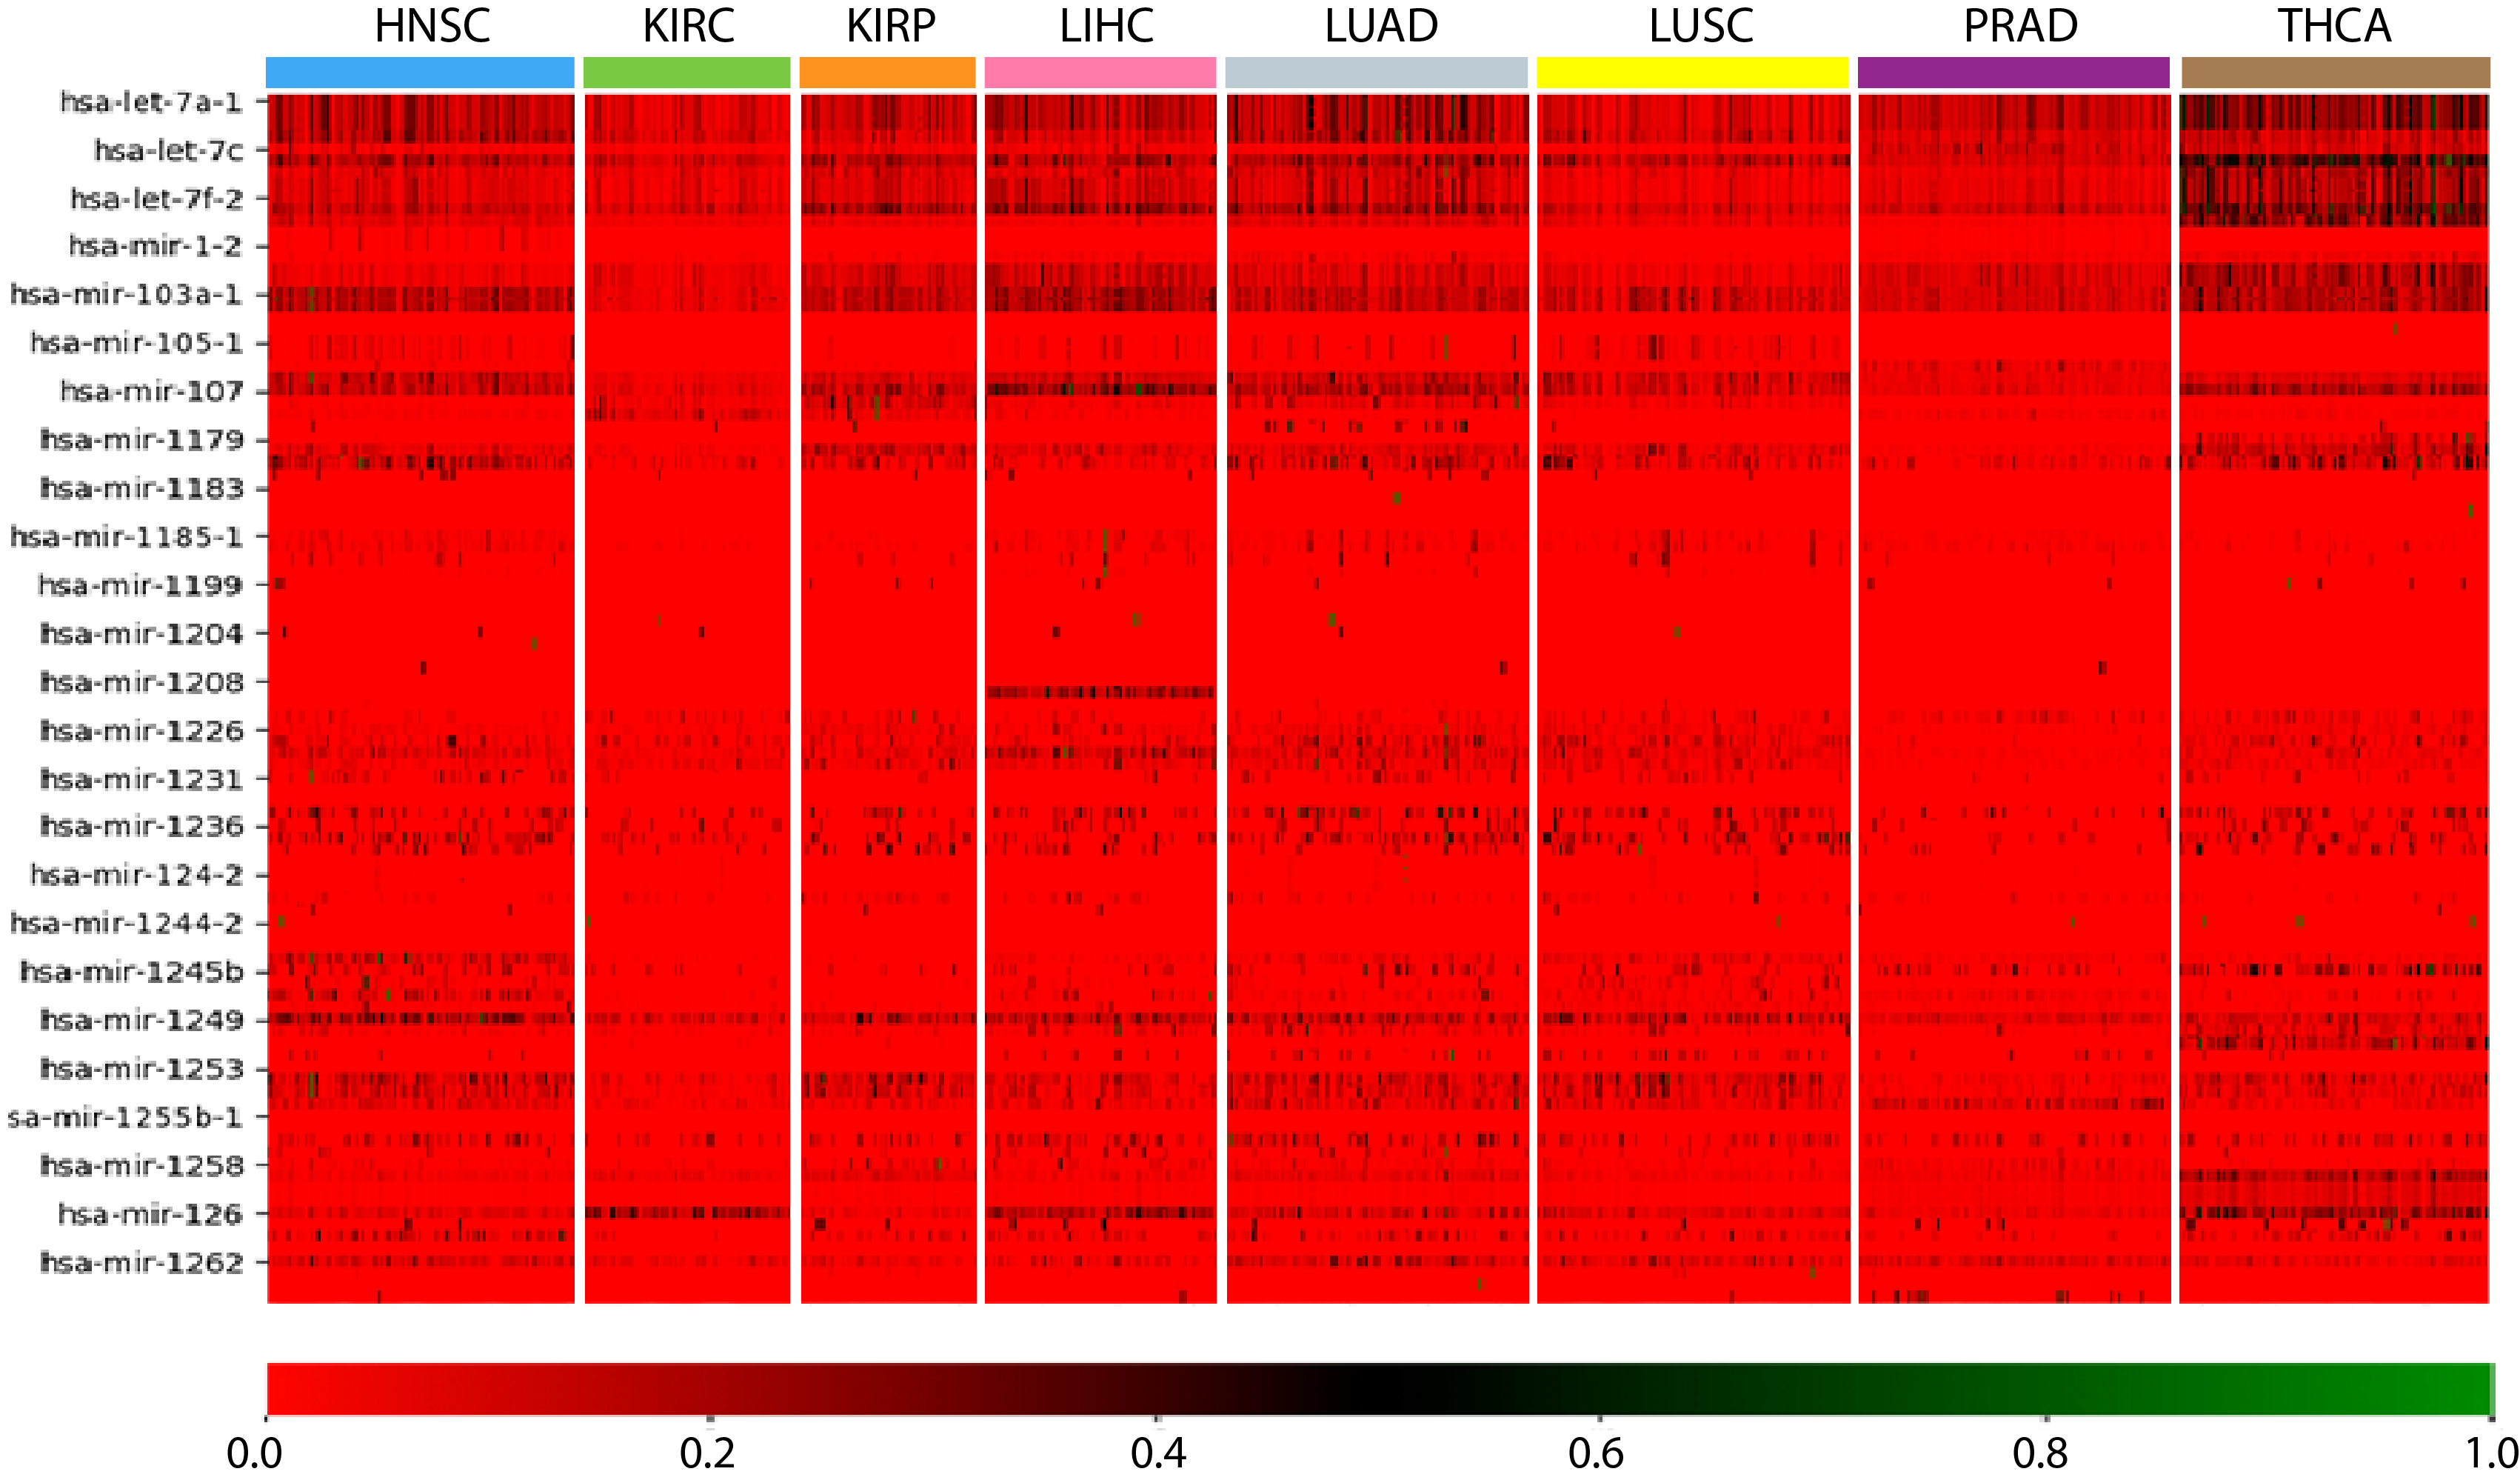
\includegraphics[width=\textwidth]{img/expmirna.png}
    \noindent
    \caption{Normalized miRNA expression profiles.}
    \label{fig:expmirna}
\end{figure}

\subsubsection{Dataset}

The expression profiles of the transcriptome expression data had the input feature dimensionality of all assayed genes and miRNA molecules. The miRNA-seq expression data contained the normalized expression counts of 1881 miRNA molecules, while the RNA-seq expression data contained the normalized expression counts of 60484 genes. As a result, the processed miRNA-seq data produced data matrix $M \in {\rm I\!R}^{1881 \; \times \; n}$, and the processed RNA-seq data produced data matrix $R \in {\rm I\!R}^{60484 \; \times \; n}$.

\subsection{Simple Nucleotide Variation}

\subsubsection{Preprocessing}

The simple nucleotide variation (SNV) data was obtained in the form of masked somatic mutations, derived from a MuTect2 Variant Aggregation and Masking workflow \cite{cibulskis2013sensitive}. The SNV data is summarized on Fig. \ref{fig:snvstats}. In \ref{fig:snvstats}a, a boxplot of the accumulated gene mutations is shown for each cancer class. Fig. \ref{fig:snvstats}b shows a stacked barplot of the distribution of genetic variations for each cancer class. Fig \ref{fig:snvstats}c shows a barplot of the somatic mutations. Somatic mutations are represented using the ($>$) symbol to denote an alteration from nucleotide X to nucleotide Y as X$>$Y. Lastly, in Fig. \ref{fig:snvstats}d, the variant distribution of the top ten mutated genes are illustrated as a series of stacked barplots organized in ascending order by the most frequently mutated genes. 

\begin{figure}[h!]
    \centering
    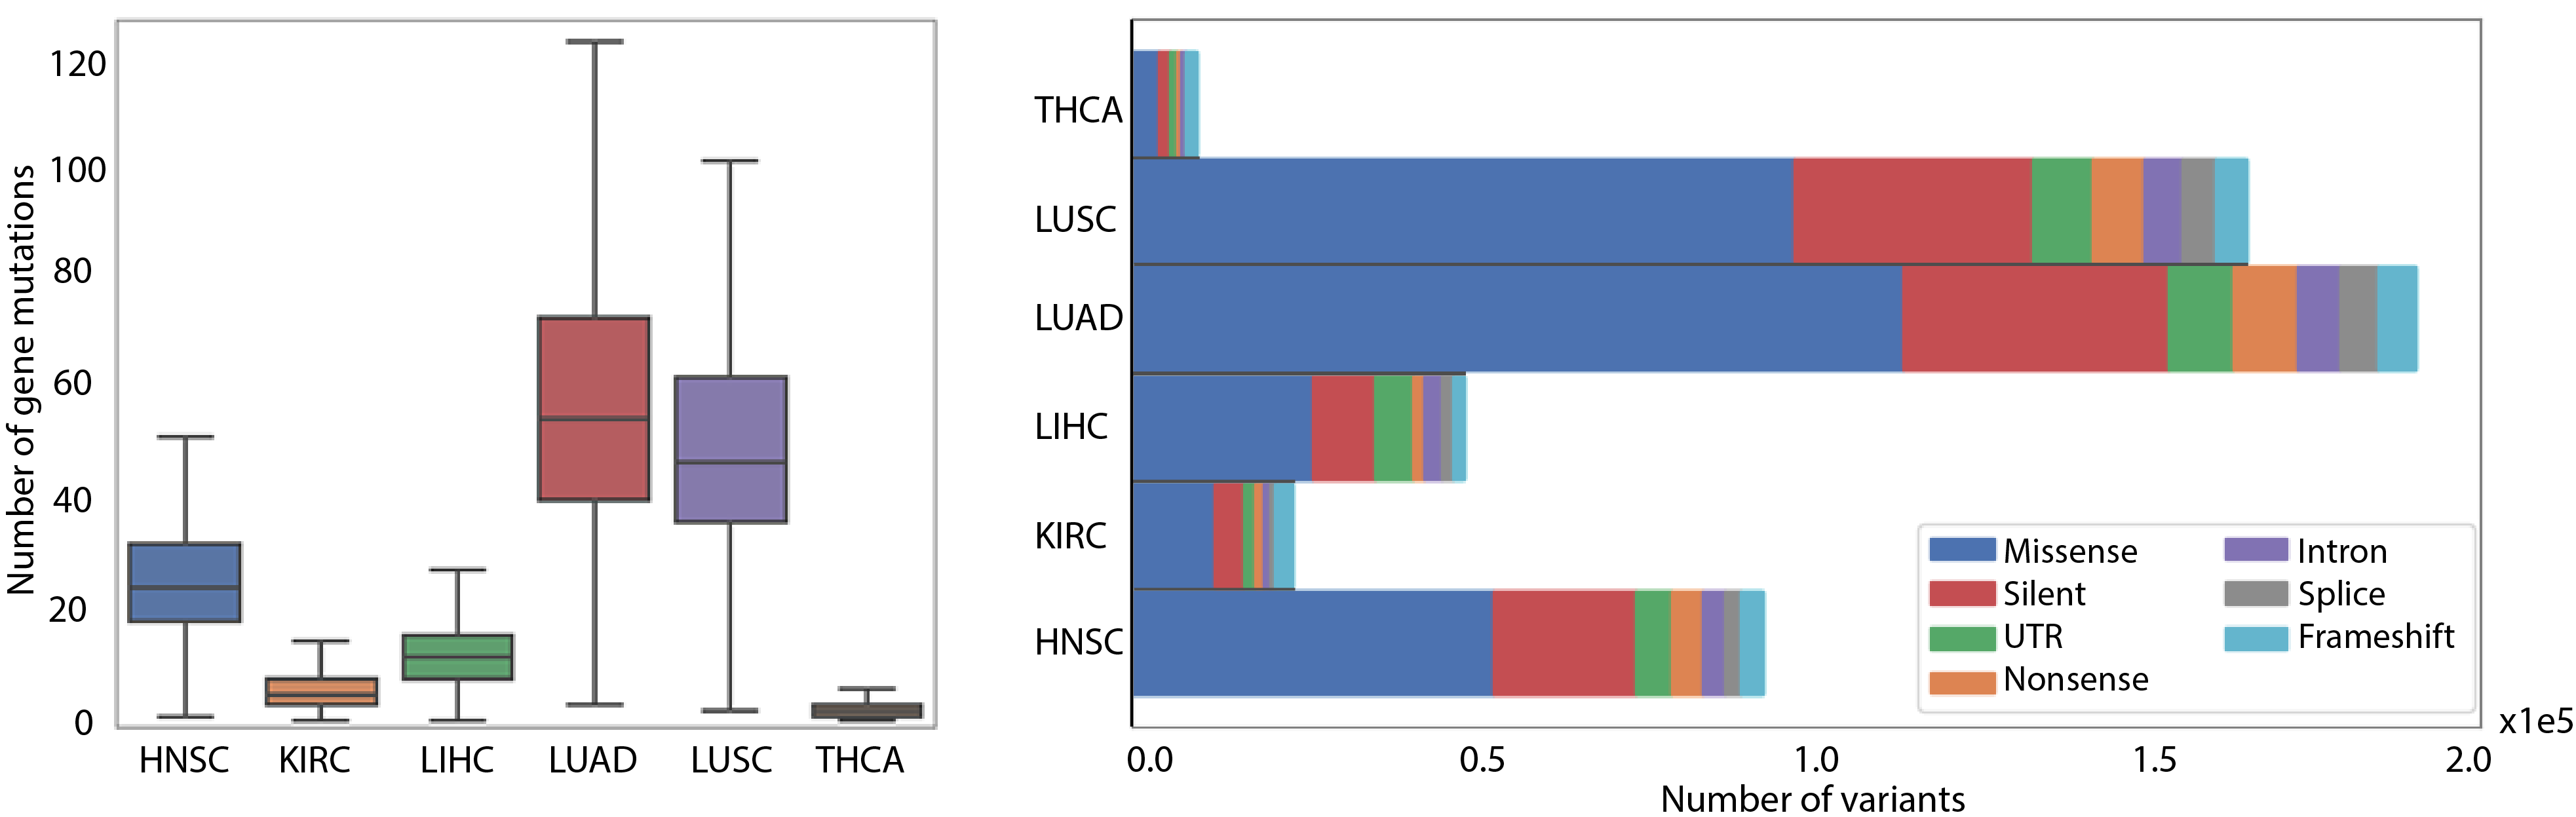
\includegraphics[width=\textwidth]{img/snvstats.png}
    \noindent
    \begin{minipage}[t]{.39\textwidth}
    \raggedright
        a) Accumulated gene mutations
    \end{minipage}% 
    \hspace{1cm}
    \begin{minipage}[t]{.5\textwidth}
        b) Variant classification distribution
    \end{minipage}
    \centering
    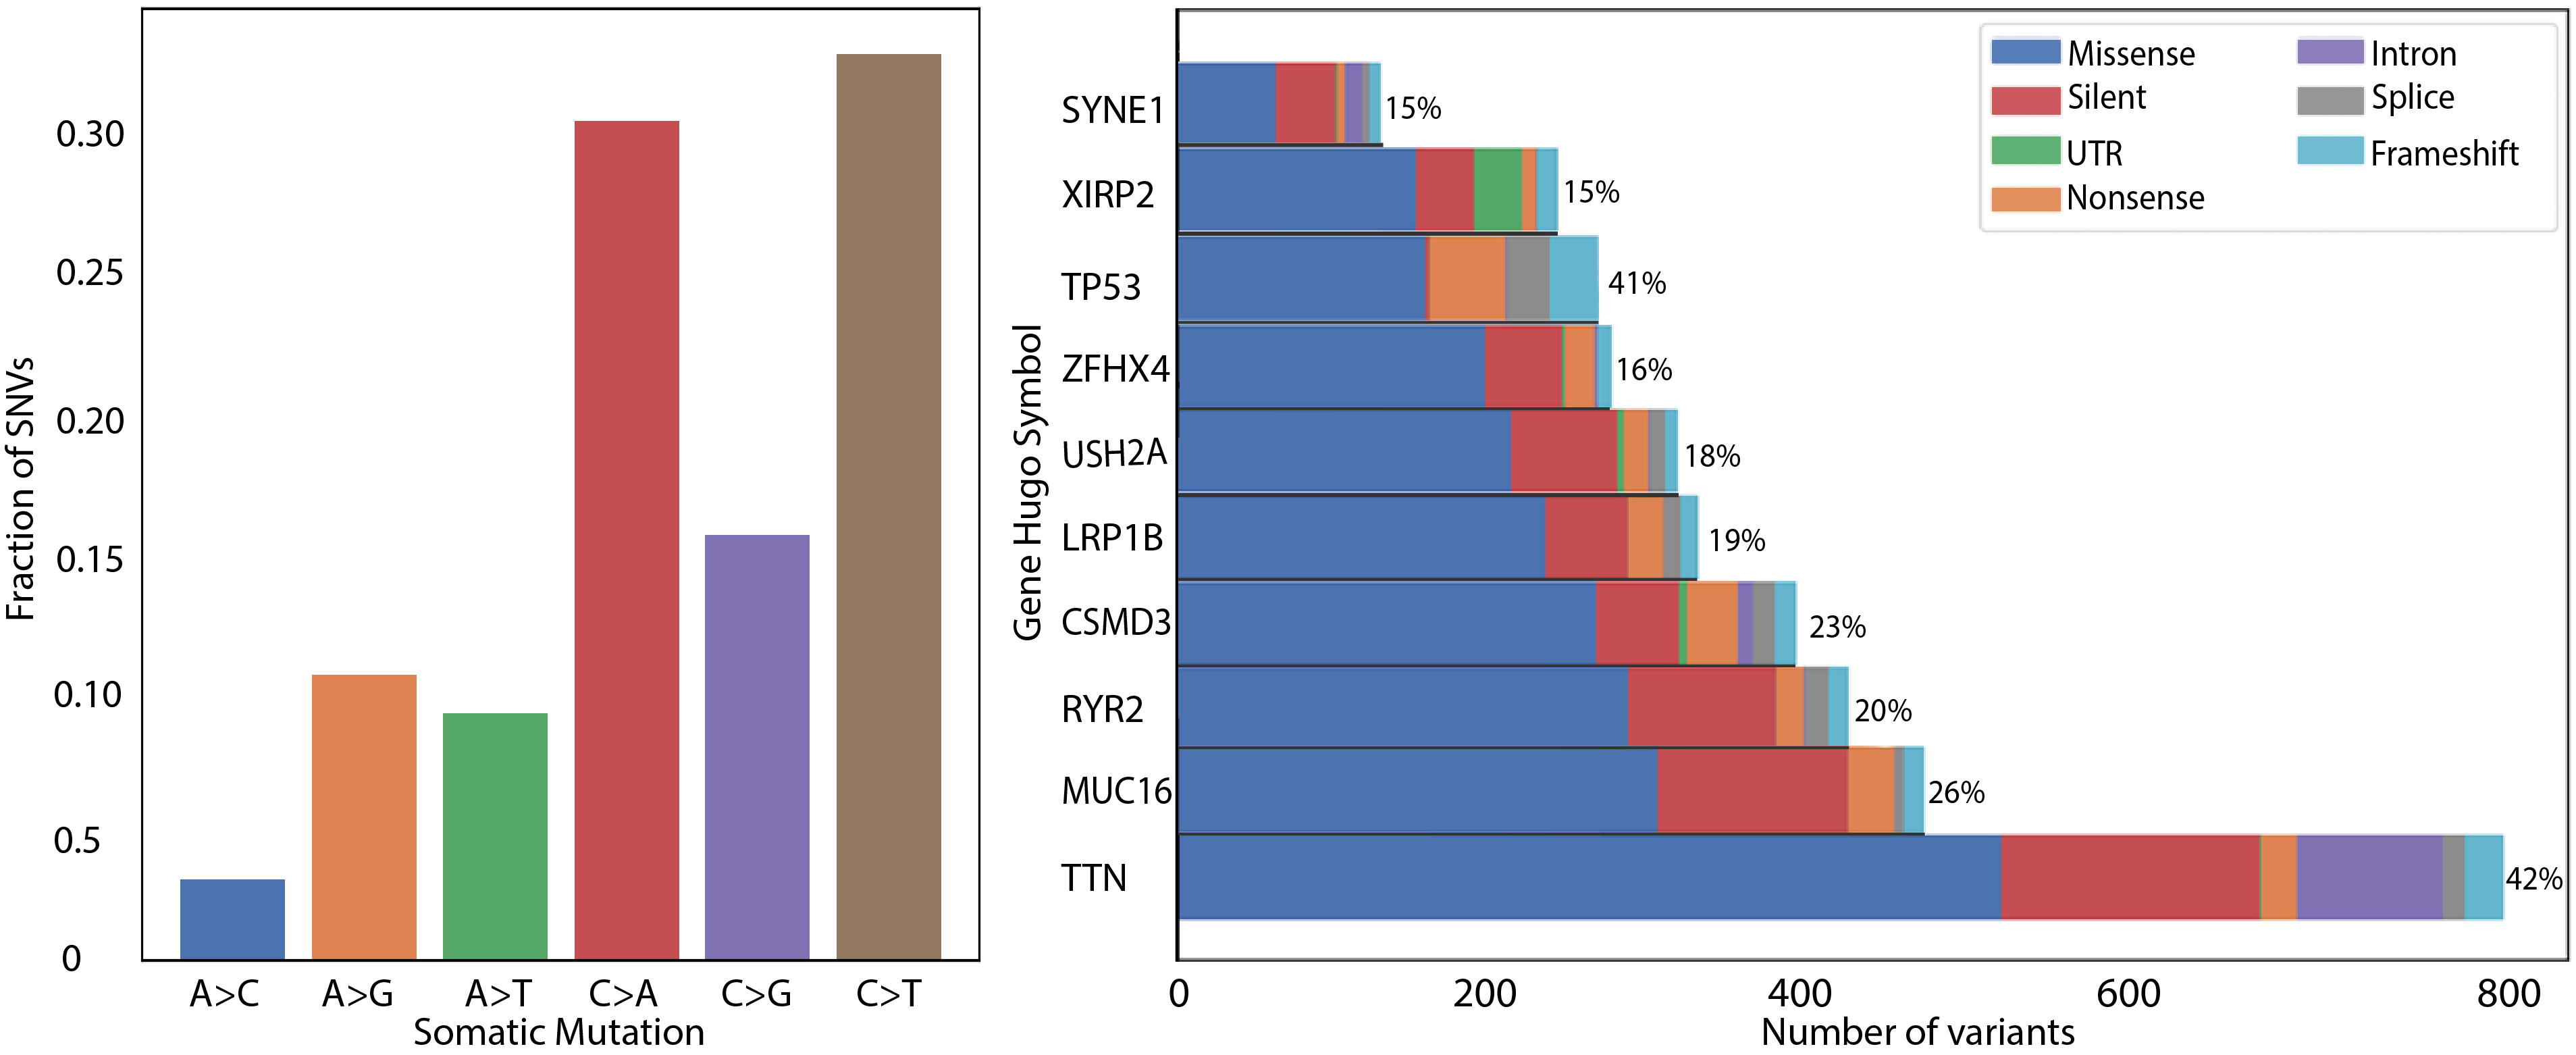
\includegraphics[width=\textwidth]{img/snvstats2.png}
    \noindent
    \begin{minipage}[t]{.39\textwidth}
    \raggedright
        c) Fraction of somatic muations
    \end{minipage}% 
    \hspace{1cm}
    \begin{minipage}[t]{.5\textwidth}
        d) Variant distribution of top 10 mutated genes
    \end{minipage}
    \caption{a) Box plot of accumulated gene mutations for each cancer type. b) Stacked bar plot showing the distribution of variant classification for each cancer type. c) Bar plot showing the fraction of all somatic mutations. d) Stacked bar plot detailing the distribution of the top 10 mutated genes.}
    \label{fig:snvstats}
\end{figure}

In this study, the analysis of the raw SNV data was based on the variant occurrence frequency of the genetic data. Variation occurence was mapped to every listed gene for all available cell samples. This was performed by mapping mutated genes to cell sample IDs in the raw SNV data, and accumulating the number of mutations for each respective cell sample.

\subsubsection{Dataset}

After preprocessing the SNV data, the variant occurrence frequency was obtained for 20516 human genes for each cell mass sample. The variant occurrence frequency was recorded in matrix $S \in \{\mathbb{Z}_{\geq 0}\}^{20516 \; \times \; m}$, where the 20516 rows coorespond to genes, and the m columns correspond to the m cell samples per gene. Accordingly, an entry of the matrix $S$ indicates the number of mutations observed for a cell on a given gene. 

\section{Dimensionality Reduction}

In the following, we describe the various forms of dimensionality reduction used to deal with the high dimensionality of the genomic data and the selection of relevant features. 

\subsection{Stacked Denoising Autoencoder}

%If descriving the model use a present tense, leave the experimental parameters for later

A SDAE was used to acquire compressed feature vectors from all genomic data sources. A two layer SDAE with dimensions 1000, and 500 was trained using a designated training set. Optimal model parameters were selected based on model performance during 10-fold cross validation. Post training, a layer with reduced dimensionality and a low cross validation error was selected. The defined objective here was to acquire a reduced mapping that encodes the original data with minimal loss of meaningful patterns.

%Product of the weight matrix,
%Pliral for the weight matricies
%Multiple the matrcies of the layers 

\subsection{Deeply Connected Genes}

In our experiments, the weights of the trained SDAE were used to extract the raw features most strongly connected to the reduced subspace for CNV, RNA-seq and miRNA-seq data sources. These features were extracted from the SDAE by computing the product of the weight matrices for each layer \cite{danaee2017deep}. 
The product of the weights for each layer in the trained and optimally parametized SDAEs were observed to be highly normally distributed as shown in Fig. \ref{fig:zscoreHist}. 

\begin{figure}[h!]
     \centering
         \centering
         \sidesubfloat[]{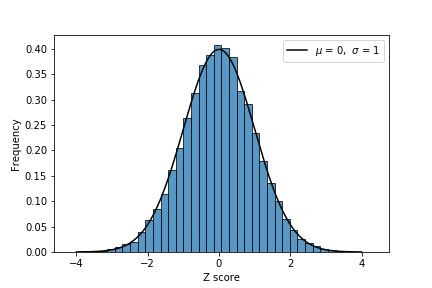
\includegraphics[width=0.25\textwidth]{img/zscoreCNV.png}}
     \hfill
         \centering
         \sidesubfloat[]{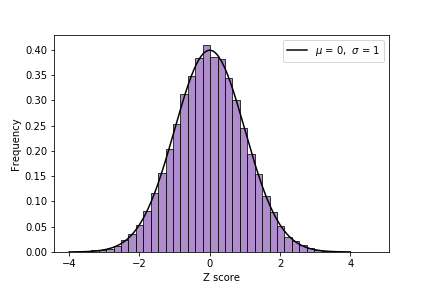
\includegraphics[width=0.25\textwidth]{img/zscoreRNA.png}}
     \hfill
         \centering
         \sidesubfloat[]{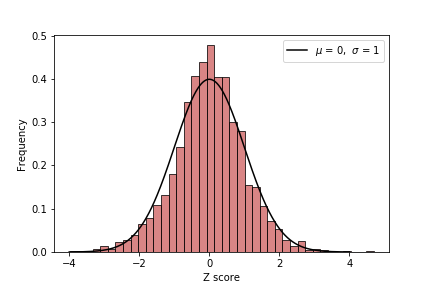
\includegraphics[width=0.25\textwidth]{img/zscoreMIRNA.png}}

        \caption{Histogram of z-scores from dot product of SDAE weight matrices for (a) CNV (b) RNA-seq and (c) miRNA-seq.}
        \label{fig:zscoreHist}
\end{figure}

The most statistically significant features were identified by fitting the weight matrices to a normal distribution, and computing a p value to select features that match the preselected experimental dimensions.

\subsection{Differential Expression}

For the transcriptome expression data, deferentially expressed genes were identified, and utilized as features. The log$_{2}$(fold change) was computed between the median tumour cell mass expression and healthy cell mass expression. The most statistically significant features were identified by fitting the differential expression to a Guassian distribution and computing a two-tailed p-value. Features that match the preselected experimental dimensions were acquired by selecting the top most significant deferentially expressed genes using the two-tailed p-values. 

\begin{figure}[h!]
     \centering
         \centering
         \sidesubfloat[]{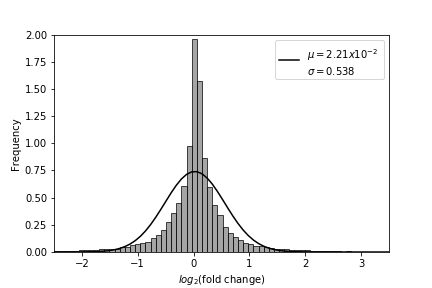
\includegraphics[width=0.4\textwidth]{img/rnaDE.png}}
     \hfill
         \centering
         \sidesubfloat[]{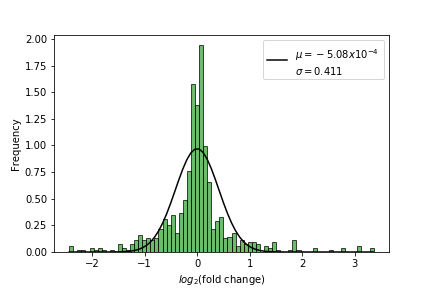
\includegraphics[width=0.4\textwidth]{img/mirnaDE.png}}
        \caption{Differential expression $log_2$(fold change) and Gaussian fit for (a) RNA-seq and (b) miRNA-seq.}
        \label{fig:deHist}
\end{figure}

\subsection{Clustered Gene Filtering}

Due to the sparse nature of the discrete point mutation SNV data, clustered gene filtering (CGF) was used to select a subset of the most discriminatory genes based on the variant occurrence frequency matrix $S$ \cite{yuan2016deepgene}. The procedure involves filtering the genes into groups based on a similarity criteria, and then selecting a subset of genes from each group that have the highest mutation frequency because these are likely of more interest. Dimensionality reduction can be controlled algorithmically through the modulation of distance threshold $d_{cgf}$, and the group element threshold $n_{cgf}$. The distance threshold dictates how similiar the mutation profiles of two genes need to be to be grouped together. The group element threshold is the number of genes kept from each group. The CGF algorithm used is summarized in Algorithm \ref{alg:cgf}.

{\singlespacing
\begin{algorithm}
\caption{Clustered Gene Filtering}\label{alg:cgf}
\begin{algorithmic}[1]
\Require Data matrix $S \in \{\mathbb{Z}_{\geq 0}\}^{p \; \times \; m}$
\Require Distance threshold $d_{cgf} > 0$, and group element threshold $n_{cgf} > 0$
\Procedure{CGF}{$S,d_{cgf},n_{cgf}$}%\Comment{The g.c.d. of a and b}
\State $S_{sum} \gets sum(S, axis=2) $\label{alg:sumA}
\State $S_{sum}^{*} \gets sort(S_{sum}, \textrm{order}=descending)$
\State $S \gets reindex(S, \textrm{index} = S_{sum}^{*})$
\State $g = 0_{1,p}$\label{alg:igsGroup}
\State $\textrm{groupNum} \gets 0$
\For{$i \in \{1 \dotsc p\}$}\label{alg:igsS}
    \If{$g_i = 0$}
        \State $\textrm{groupNum} \gets \textrm{groupNum} + 1$
        \State $g_i = \textrm{groupNum}$
        \For{$j \in \{2 \dotsc p\}$}
            \If{$j \neq i \;\; \textrm{and} \;\; g_{j} = 0$}
                \If{$d(S_{i...},S_{j...}) > d_{cgf}$}
                    \State $g_j = \textrm{groupNum}$
                \EndIf
            \EndIf
        \EndFor    
    \EndIf
\EndFor\label{alg:igsE}
\State $g_{out} \gets \varnothing$\label{alg:igsOut}
\For{$k \in \{1 \dotsc max(g)\}$}
    \For{$\textrm{all} \;\; g_c = k$}
        \If{$g_c > n_{cgf}$}
            \State $g_{out} \gets g_{out} \cup g_{c}[1 \dotsc n_{cgf}]$
        \EndIf
    \EndFor
\EndFor

\State $S_{cgf} \gets S[g_{out},:]$
\State \textbf{return} $S_{cgf}$%\Comment{The gcd is b}
\EndProcedure
\end{algorithmic}
\end{algorithm}}

\noindent
In line \ref{alg:sumA}, we sum matrix $S$ by its second dimension, such that $S_{sum} = \sum_{j} S_{ij}$ is a one dimensional vector of length $p$. We then produce $S_{sum}^{*}$ by sorting matrix $S_{sum}$ in descending order. The matrix $S$ is then reindexed to match the sorted array so that the genes with the highest mutation frequency are listed first. Line \ref{alg:igsGroup} initializes a $p$-dimensional array to store the value of the clustered group for each gene. In steps \ref{alg:igsS} to \ref{alg:igsE}, the genes of matrix $S$ are clustered by inter-gene similarity. The similarity metric between two genes $A$ and $B$ is calculated using the cosine similarity:

\begin{equation}
    d(A,B)= \frac{AB^{T}}{\lVert A \rVert \lVert B \rVert}
\end{equation}

\noindent
In line \ref{alg:igsS}, the index $i$ iterates through the $p$ genes, starting with the gene with the highest mutation frequency $S_1$.  The similarity between this gene and all the remaining genes are calculated, and if the similarity is larger than the threshold $d_{cgf}$, the respective gene is assigned to the group of $S_1$. After the similarity between $S_1$ is computed with all genes, the inter-sample similarity calculations and gene group assignment is repeated for the next ungrouped element in $S$. The last step forms the discriminatory subset by selecting the top $n_{cgf}$ in each group. The indices for the discriminatory subset are stored in the variable $g_{out}$, which is initialized as an empty set in line \ref{alg:igsOut}. The following two for loops iterate through all the genes $g_c$ for a specific group $k$, and stores the top $n_{cgf}$ genes as long as the group does not have fewer then $n_{cgf}$ elements.

\section{Model Interpretation}

%\subsection{Grad-cam}

\subsection{Gene-wise Interpretable Explanations}

To find a gene-wise explanation, the LIME procedure is used to approximate the dGMU model with a linear model of class $G$, such that $g(\tilde{x}) = {w_g}^{T} \tilde{x}$. Perturbed instance $\tilde{x}$ is generated by individually noising each feature by drawing from a normal distribution. The mean and standard deviation is taken from each feature in the original dataset $X$. The perturbed instance is weighted using an exponential kernel learned over a euclidean distance by letting $\mu_{x_i}(\tilde{x}) = exp(-\sqrt{\sum_{i=1}^{n}(x - \tilde{x})^2})/\sigma)$. The kernel width $\sigma$ is defined as 0.75 times the square root of the number of training instances (default value for $\sigma$ is used as established in \cite{ribeiro2016should}). With a locally weighted squared error $J$, as defined in Eq. (\ref{eq:lime}), we learn the weights $w_g$ of the sparse linear model via least squares. Each trained model provides interpretable explanations through the learned weights. The magnitude of a coefficient relates to the importance of the respective gene in sample $x_i$. Furthermore, genes with a positive weight coefficient are positively correlated with the prediction of the dGMU model and genes with a negative weight coefficient are negatively correlated. Accordingly, the explanation of a single prediction provides an interpretable framework by indicating the genes that were most influential. And more specifically, by indicating how the RNA-seq expression or SNV of the gene correlates with the model prediction. 

The gene-wise explanations for a single prediction provides locally faithful insight into the logic of the classifier. In order to assess the global fidelity of the model, gene-wise explanations are pooled to evaluate the reliability of the predictions as a whole. Gene-wise explanations are extended to understand the set of individual instances associated with correctly labelled predictions. Explanations for a set of correctly labelled instances are relevant in understanding the reliability of the classifier and assessing how the model behaves globally. Given the dataset of correctly labelled instances for cancer class $k$, $\mathcal{X}_k$, we construct an $n \times p$ dimensional explanation matrix by setting $\mathcal{W}_{ij} = \xi(\mathcal{X}_k)$. The matrix $\mathcal{W}_{ij}$ represents the local importance of all $n$ genes for each of the $p$ correctly labelled instances for a given class. The gene-wise global weights can then be pooled in an $n$ dimensional vector g = $\sum_{i=1}^{n}\mathcal{W}_{ij}$. Accordingly, genes that explain more instances will be ranked with a higher importance.


    \chapter{Experimental Results} \label{chap:results}

\section{Experiment setup}
\subsection{Datasets}

In order to validate the experimental methods discussed in this thesis, various datasets we utilized as shown in Table \ref{table:expData}. 


\begin{table}[ht]
\caption{Summary of experimental datasets} % title of Table
\centering % used for centering table
\begin{tabular}{l l l l l l} % centered columns (4 columns)
\hline %inserts single horizontal lines
Bimodal dataset & Method & Samples & Classes & Learning task & Feature type \\ %[0.5ex] % inserts table
%heading
\hline % inserts single horizontal line
RNA-seq + miRNA-seq & SDAE & 3988 & 9 & classification & real\\ 
RNA-seq + miRNA-seq & DCF & 3988 & 9 & classification & real\\ 
RNA-seq + miRNA-seq & DE & 3988 & 9 & classification & real\\ 
CNV + RNA-seq & DCF & 3988 & 9 & classification & real\\ 
CNV + RNA-seq & SDAE & 3988 & 9 & classification & real\\ 
miRNA-seq + SNV & DCF & 3375 & 6 & classification & real + integer\\ miRNA-seq + SNV & SDAE & 3375 & 6 & classification & real + integer\\ 
%Exp7 & dp & fet & - & regression     & real\\ 
[1ex]   % [1ex] adds vertical space 
\hline %inserts single line
\end{tabular}
\label{table:expData}
\end{table}

\section{Results}

In the following, we report the results from all experiments. In all cases, experiments were constructed using the following experimental settings and constraints:

\begin{itemize}
    \item The datasets were divided into a 60/20/20 split for training, validation, and testing, respectively.
    \item Hyperparameter tuning was performed on the cross validation set.
    \item Experiments were repeated 10 times using 10 fold cross validation on the training set.
\end{itemize}

\subsection{miRNA-seq + RNA-seq}\label{subsub:m_r_SDAE}

\subsubsection{SDAE}

\begin{figure}[H]
     \centering
     \begin{subfigure}[b]{0.49\textwidth}
         \centering
         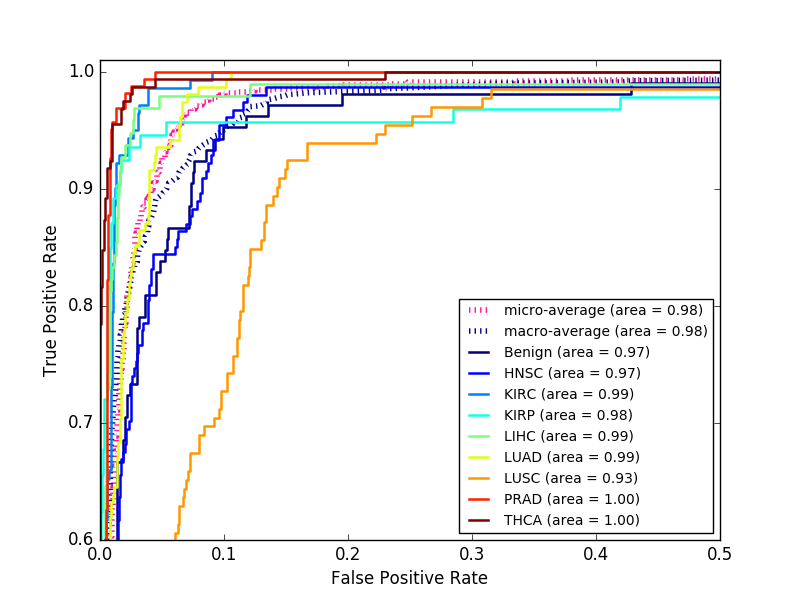
\includegraphics[width=\textwidth]{img/m_r/m_r_sdae_dgmu_roc.png}
         \caption{}
     \end{subfigure}
     \hfill
     \begin{subfigure}[b]{0.49\textwidth}
         \centering
         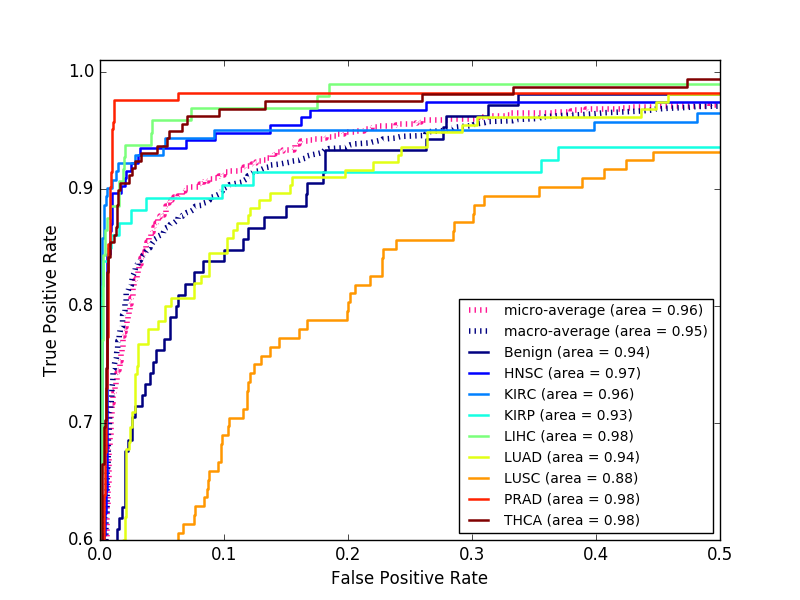
\includegraphics[width=\textwidth]{img/m_r/m_r_sdae_gmu_roc.png}
         \caption{}
     \end{subfigure}
     \hfill
     \begin{subfigure}[b]{0.49\textwidth}
         \centering
         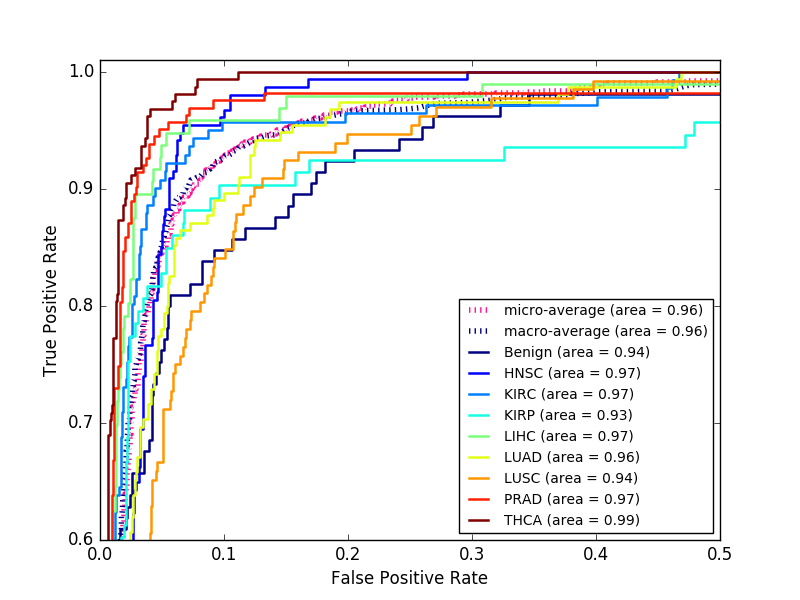
\includegraphics[width=\textwidth]{img/m_r/m_r_sdae_mlp_roc.png}
         \caption{}
     \end{subfigure}
     \begin{subfigure}[b]{0.49\textwidth}
         \centering
         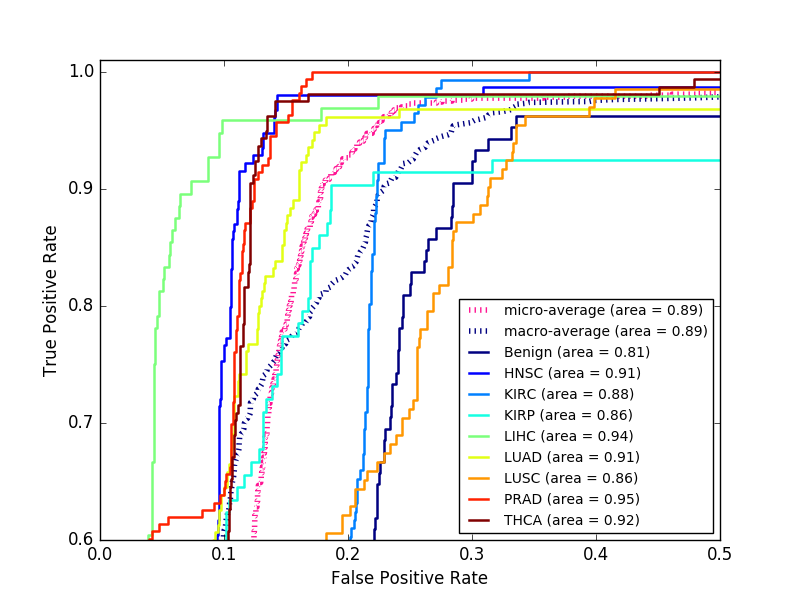
\includegraphics[width=\textwidth]{img/m_r/m_r_sdae_moe_roc.png}
         \caption{}
     \end{subfigure}
        \caption{miRNA-seq and RNA-seq SDAE bimodal model ROC plots for a) dGMU b) GMU c) MLP and d) ME.}
        \label{fig:m_r_sdae_roc}
\end{figure}

\begin{table}[H]
   \caption{Summary of classification agreement for miRNA-seq and RNA-seq SDAE reduced to 500 features.} 
   \small % text size of table content
   \centering % center the table
   \begin{tabular}{lllll} % alignment of each column data
   \toprule[\heavyrulewidth]\toprule[\heavyrulewidth]
   \textbf{Modality} & \textbf{Accuracy} & \textbf{Precision} & \textbf{Recall} & \textbf{F1-score} \\ 
   \midrule
   \multicolumn{1}{l}{\textbf{Bimodal}} \\
        dGMU & 0.9206 &	0.9218 & 0.9196	& 0.9207\\
        GMU  & 0.9123 &	0.9123 & 0.9123 & 0.9123\\
        MoE  & 0.8817 &	0.8813 & 0.8760 & 0.8786\\
        MLP  & 0.8829 &	0.8816 & 0.8750 & 0.8783\\
        SVM  & 0.8480 &	0.8444 & 0.8404 & 0.8424\\
   \midrule
   \multicolumn{1}{l}{\textbf{miRNA-seq}} \\
        MLP  & 0.8999 &	0.9020 & 0.8960 & 0.8990\\
        SVM  & 0.8673 &	0.8902 & 0.8592 & 0.8744\\
   \midrule
   \multicolumn{1}{l}{\textbf{RNA-seq}}  \\
        MLP  & 0.8361 &	0.6799 & 0.8379 & 0.8311\\
        SVM  & 0.8430 &	0.8381 & 0.8349 & 0.8365\\
   \bottomrule[\heavyrulewidth] 
   \end{tabular}
   \label{table:m_r_sdae_exp41}
\end{table}

\begin{figure}[H]
     \centering
     \begin{subfigure}[b]{\textwidth}
         \centering
         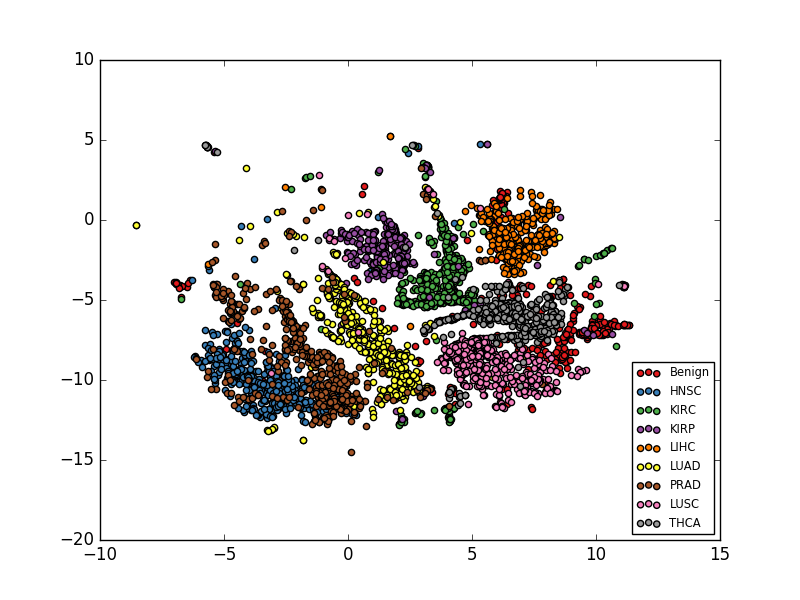
\includegraphics[width=\textwidth]{img/m_r/m_r_sdae_tsne.png}
     \end{subfigure}
        \caption{miRNA-seq and RNA-seq SDAE dGMU model latent space clustered with t-distributed stochastic neighbor embedding (t-SNE).}
        \label{fig:r_m_sdae_tsne}
\end{figure}

\subsubsection{DCF}

\begin{figure}[H]
     \centering
     \begin{subfigure}[b]{0.49\textwidth}
         \centering
         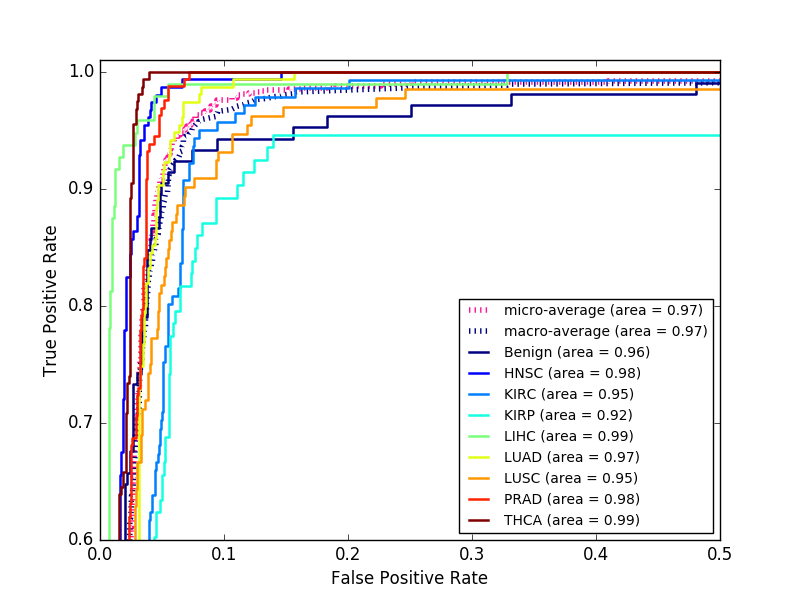
\includegraphics[width=\textwidth]{img/m_r/m_r_dcf_dgmu_roc.png}
         \caption{}
     \end{subfigure}
     \hfill
     \begin{subfigure}[b]{0.49\textwidth}
         \centering
         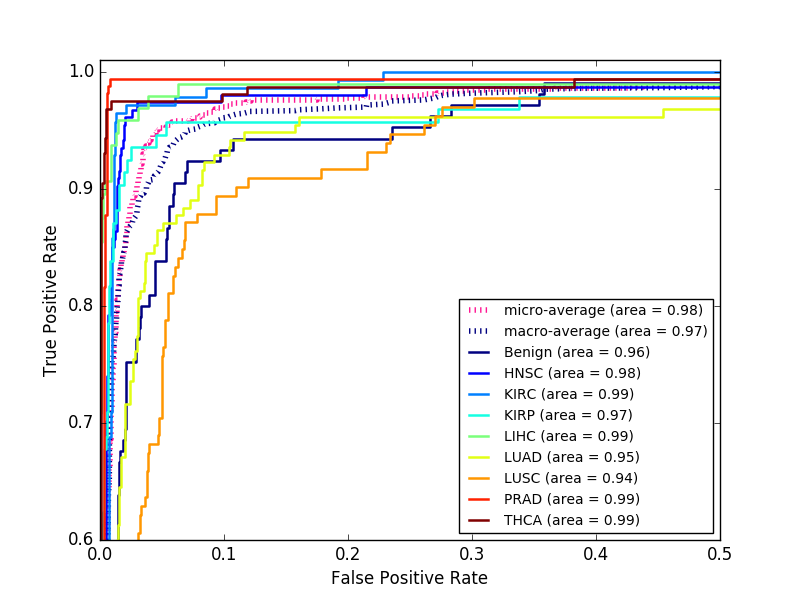
\includegraphics[width=\textwidth]{img/m_r/m_r_dcf_gmu_roc.png}
         \caption{}
     \end{subfigure}
     \hfill
     \begin{subfigure}[b]{0.49\textwidth}
         \centering
         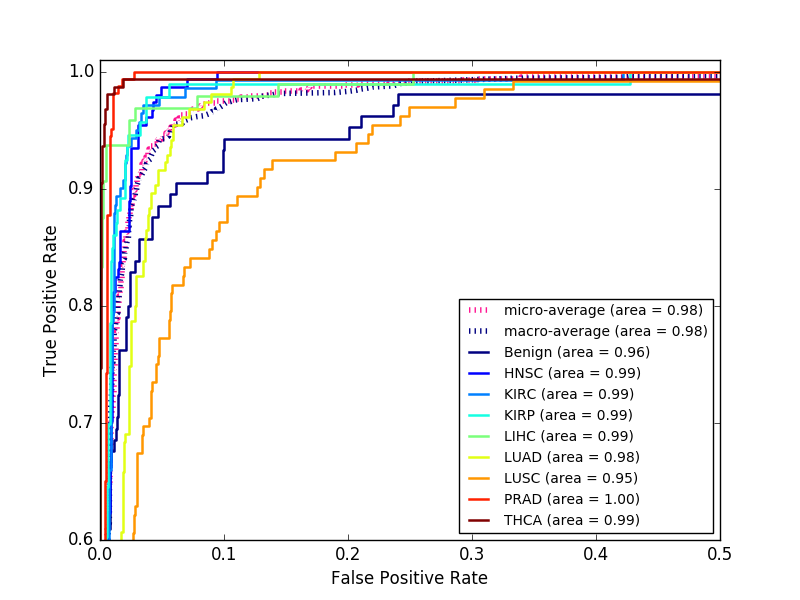
\includegraphics[width=\textwidth]{img/m_r/m_r_dcf_mlp_roc.png}
         \caption{}
     \end{subfigure}
     \begin{subfigure}[b]{0.49\textwidth}
         \centering
         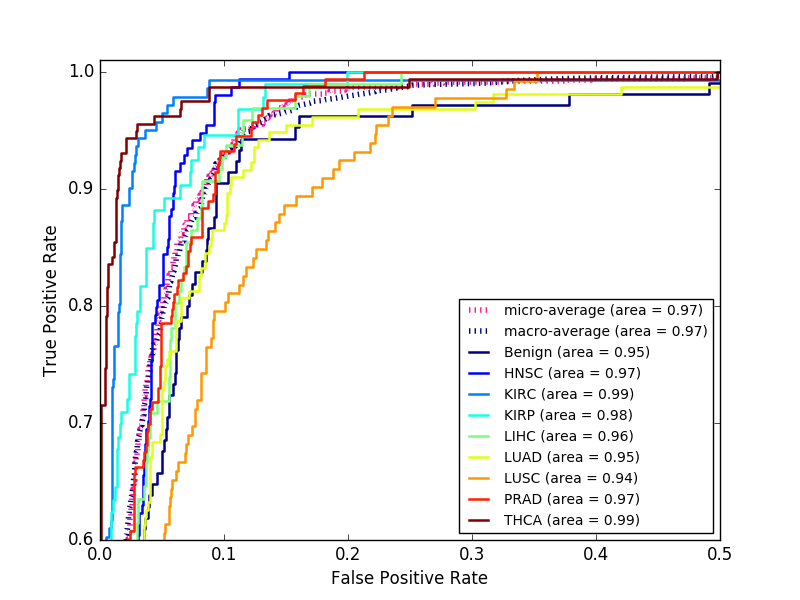
\includegraphics[width=\textwidth]{img/m_r/m_r_dcf_moe_roc.png}
         \caption{}
     \end{subfigure}
        \caption{miRNA-seq and RNA-seq DCF bimodal model ROC plots for a) dGMU b) GMU c) MLP and d) ME.}
        \label{fig:m_r_dcf_roc}
\end{figure}

\begin{table}[H]
   \caption{Summary of classification agreement for miRNA-seq and RNA-seq DCF reduced to 500 features.} 
   \small % text size of table content
   \centering % center the table
   \begin{tabular}{lllll} % alignment of each column data
   \toprule[\heavyrulewidth]\toprule[\heavyrulewidth]
   \textbf{Modality} & \textbf{Accuracy} & \textbf{Precision} & \textbf{Recall} & \textbf{F1-score} \\ 
   \midrule
   \multicolumn{1}{l}{\textbf{Bimodal}} \\
        dGMU & 0.9373 &	0.9385 & 0.9094 & 0.9362\\
        GMU  & 0.9332 &	0.9332 & 0.9332 & 0.9332\\
        MoE  & 0.9106 &	0.9120 & 0.9094 & 0.9107\\
        MLP  & 0.9215 &	0.9208 & 0.9136 & 0.9148\\
        SVM  & 0.8981 &	0.9081 & 0.8922 & 0.9001\\
   \midrule
   \multicolumn{1}{l}{\textbf{miRNA-seq}} \\
        MLP  & 0.8847 &	0.8881 & 0.8815 & 0.8848\\
        SVM  & 0.8739 &	0.8806 & 0.8690 & 0.8748\\
   \midrule
   \multicolumn{1}{l}{\textbf{RNA-seq}}  \\
        MLP  & 0.9023 &	0.9024 & 0.8940 & 0.8982\\
        SVM  & 0.9068 &	0.9116 & 0.9006 & 0.9061\\
   \bottomrule[\heavyrulewidth] 
   \end{tabular}
   \label{table:m_r_dcf_exp41}
\end{table}

\begin{figure}[H]
     \centering
     \begin{subfigure}[b]{\textwidth}
         \centering
         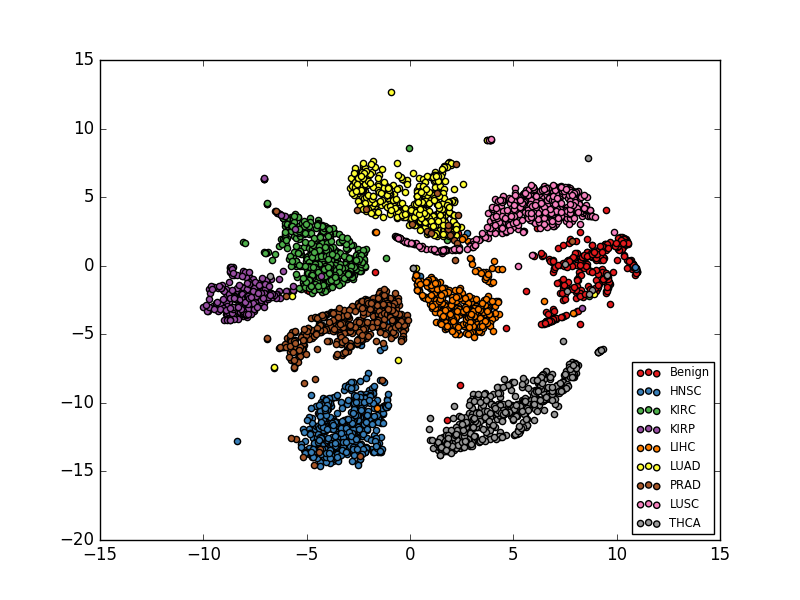
\includegraphics[width=\textwidth]{img/m_r/m_r_dcf_tsne.png}
     \end{subfigure}
        \caption{miRNA-seq and RNA-seq DCF dGMU model latent space clustered with t-distributed stochastic neighbor embedding (t-SNE).}
        \label{fig:r_m_dcf_tsne}
\end{figure}

\subsubsection{DE}

\begin{figure}[H]
     \centering
     \begin{subfigure}[b]{0.49\textwidth}
         \centering
         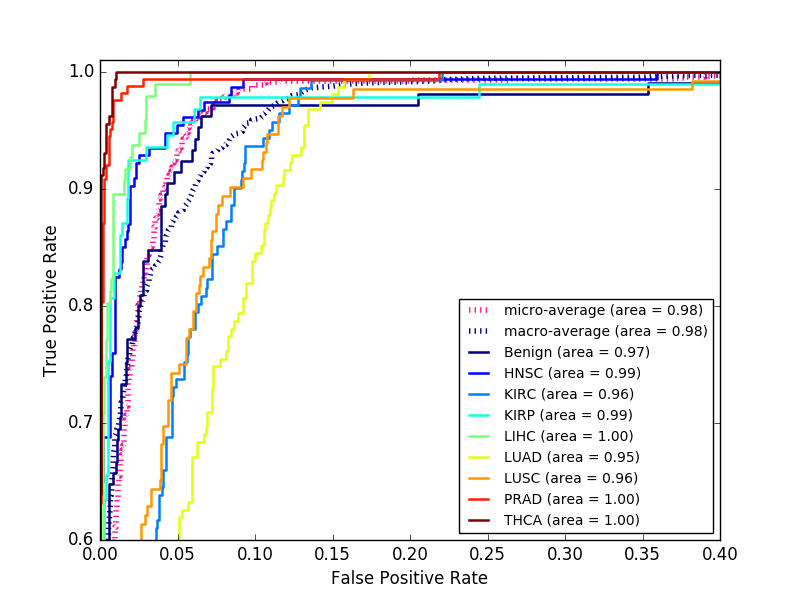
\includegraphics[width=\textwidth]{img/m_r/de_r_m_dgmu_roc.png}
         \caption{}
     \end{subfigure}
     \hfill
     \begin{subfigure}[b]{0.49\textwidth}
         \centering
         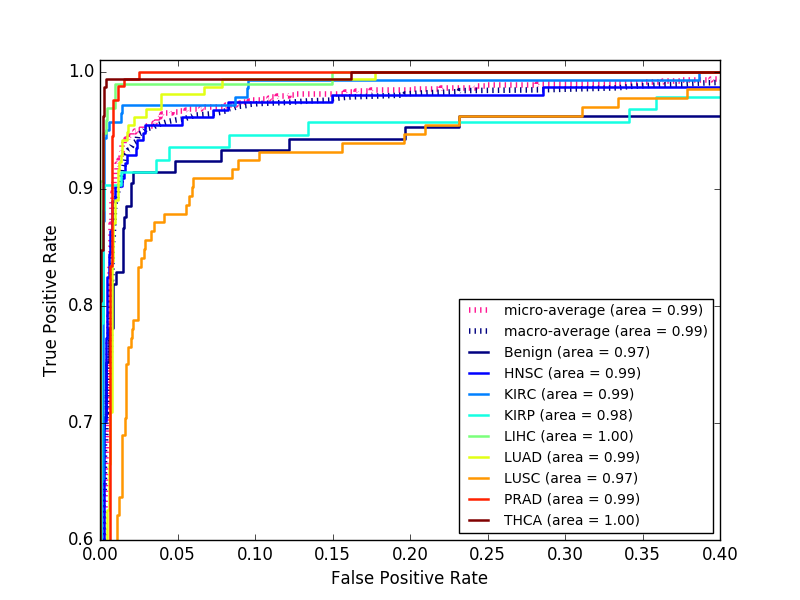
\includegraphics[width=\textwidth]{img/m_r/de_r_m_gmu_roc.png}
         \caption{}
     \end{subfigure}
     \hfill
     \begin{subfigure}[b]{0.49\textwidth}
         \centering
         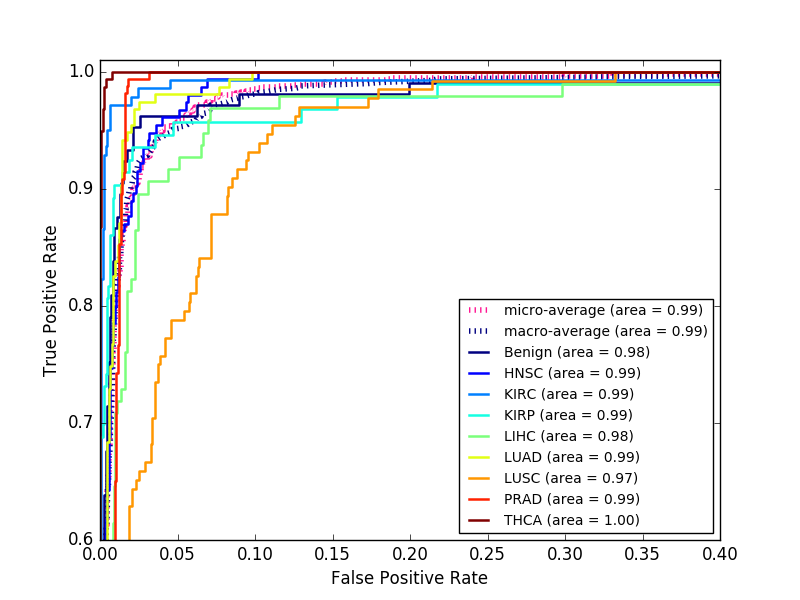
\includegraphics[width=\textwidth]{img/m_r/de_r_m_mlp_roc.png}
         \caption{}
     \end{subfigure}
     \begin{subfigure}[b]{0.49\textwidth}
         \centering
         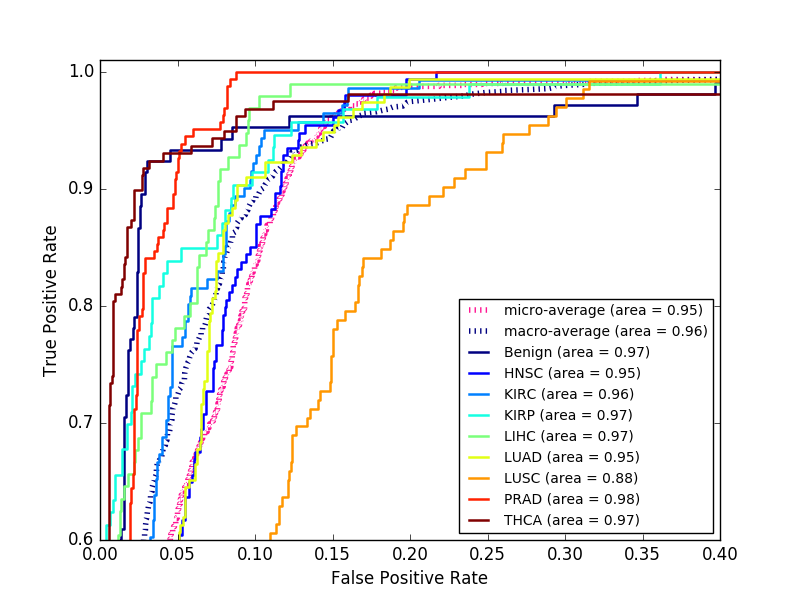
\includegraphics[width=\textwidth]{img/m_r/de_r_m_moe_roc.png}
         \caption{}
     \end{subfigure}
        \caption{miRNA-seq and RNA-seq DE bimodal model ROC plots for a) dGMU b) GMU c) MLP and d) ME.}
        \label{fig:m_r_de_roc}
\end{figure}

\begin{figure}[H]
     \centering
     \begin{subfigure}[b]{\textwidth}
         \centering
         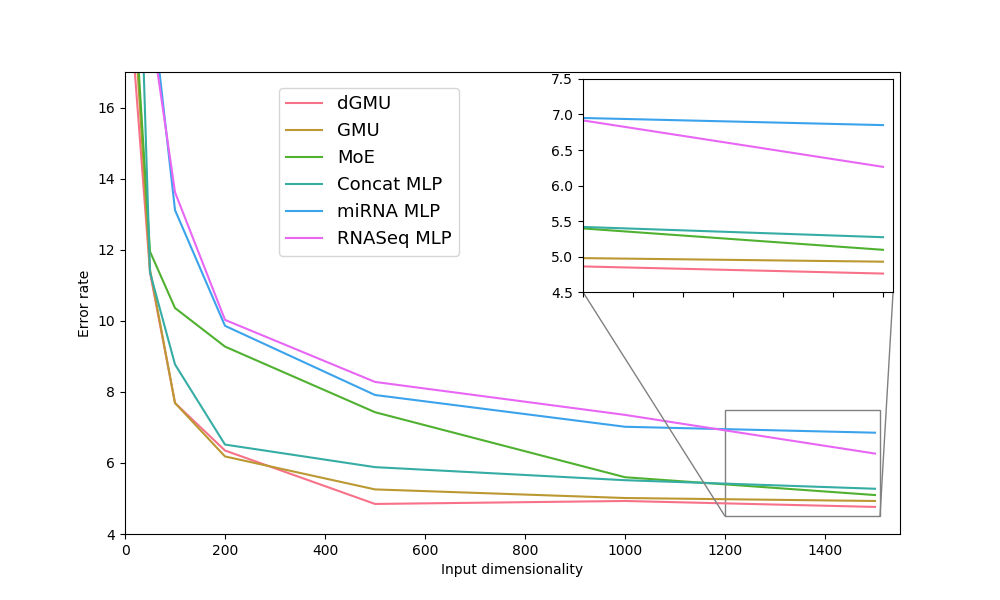
\includegraphics[width=\textwidth]{img/m_r/exp42.png}
     \end{subfigure}
        \caption{miRNA-seq and RNA-seq DE model error rates as a function of input dimensionality.}
        \label{fig:m_r_de_exp42}
\end{figure}

\begin{table}[H]
   \caption{Summary of classification agreement for miRNA-seq and RNA-seq DE reduced to 500 features.} 
   \label{tab:example_multicolumn}
   \small % text size of table content
   \centering % center the table
   \begin{tabular}{lllll} % alignment of each column data
   \toprule[\heavyrulewidth]\toprule[\heavyrulewidth]
   \textbf{Modality} & \textbf{Accuracy} & \textbf{Precision} & \textbf{Recall} & \textbf{F1-score} \\ 
   \midrule
   \multicolumn{1}{l}{\textbf{Bimodal}} \\
        dGMU & 0.9615 & 0.9533 & 0.9496 & 0.9514\\
        GMU  & 0.9475 & 0.9475 & 0.9475 & 0.9475\\
        MoE   & 0.9257 & 0.9327 & 0.9279 & 0.9298\\
        MLP  & 0.9412 & 0.9412 & 0.9401 & 0.9407\\
        SVM  & 0.9257 & 0.9238 & 0.9216 & 0.9227\\
   \midrule
   \multicolumn{1}{l}{\textbf{miRNA-seq}} \\
        MLP  & 0.9209 &	0.9158 & 0.9181 & 0.9215\\
        SVM  & 0.9150 &	0.9158 & 0.9112 & 0.9135\\
   \midrule
   \multicolumn{1}{l}{\textbf{RNA-seq}}  \\
        MLP  & 0.9172 &	0.9192 & 0.9135 & 0.9163\\
        SVM  & 0.9175 &	0.9158 & 0.9125 & 0.9141\\
   \bottomrule[\heavyrulewidth] 
   \end{tabular}
   \label{table:m_r_de_exp41}
\end{table}

\begin{figure}[H]
     \centering
     \begin{subfigure}[b]{\textwidth}
         \centering
         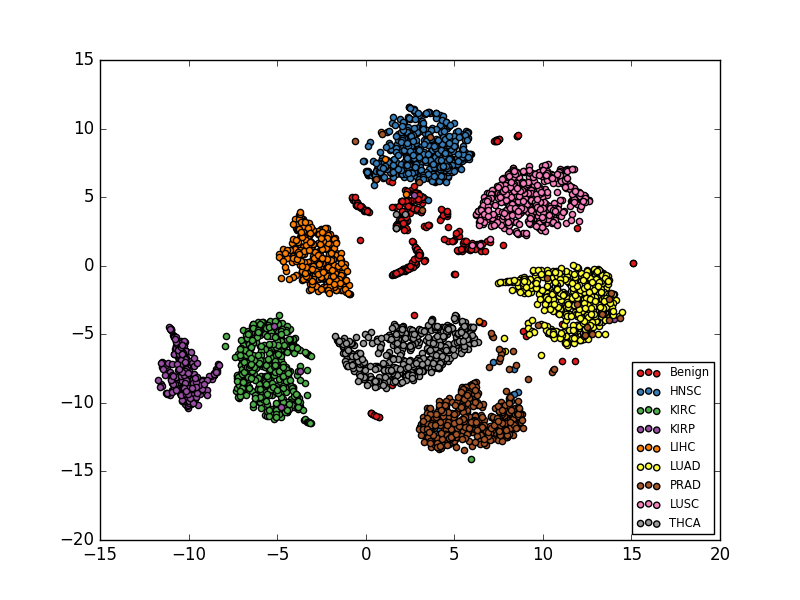
\includegraphics[width=\textwidth]{img/m_r/r_m_de_tsne.png}
         \caption{}
     \end{subfigure}
        \caption{miRNA-seq and RNA-seq DE dGMU model latent space clustered with t-distributed stochastic neighbor embedding (t-SNE).}
        \label{fig:r_m_de_tsne}
\end{figure}

%%%%%%%%%%%%%%%%%%%%%%%%%%%%%%%%%%%%%%%%%%%%%%%%%%%%%%%%%%%%%%%%%%%%%%%%%%%%%%%%%%
%c + R
%%%%%%%%%%%%%%%%%%%%%%%%%%%%%%%%%%%%%%%%%%%%%%%%%%%%%%%%%%%%%%%%%%%%%%%%%%%%%%%%%%

\subsection{CNV + RNA-seq}\label{sub:c_r_results}

\subsubsection{SDAE}

\begin{figure}[H]
     \centering
     \begin{subfigure}[b]{0.49\textwidth}
         \centering
         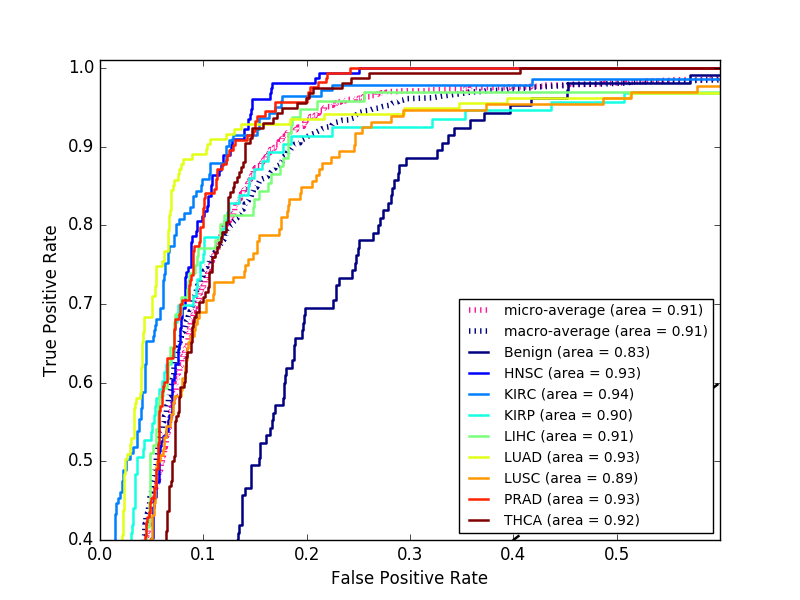
\includegraphics[width=\textwidth]{img/c_r/c_r_sdae_dgmu_roc.png}
         \caption{}
     \end{subfigure}
     \hfill
     \begin{subfigure}[b]{0.49\textwidth}
         \centering
         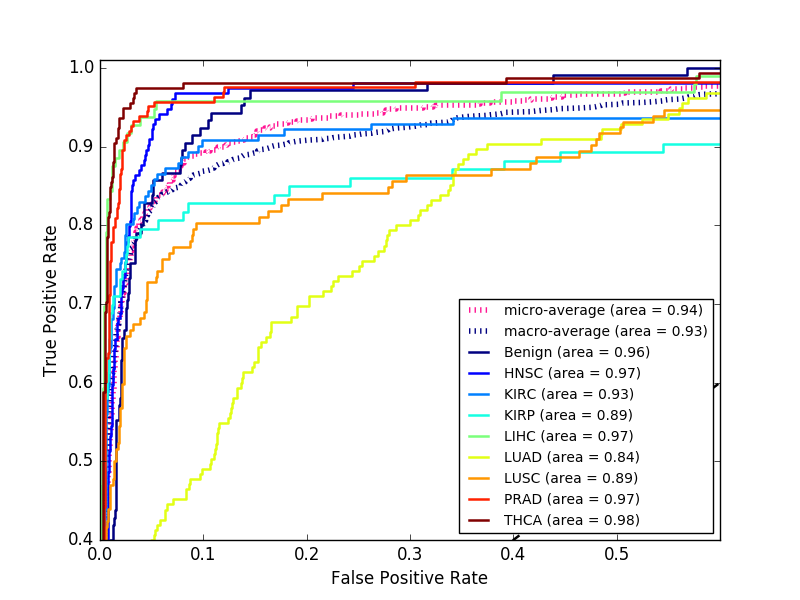
\includegraphics[width=\textwidth]{img/c_r/c_r_sdae_gmu_roc.png}
         \caption{}
     \end{subfigure}
     \hfill
     \begin{subfigure}[b]{0.49\textwidth}
         \centering
         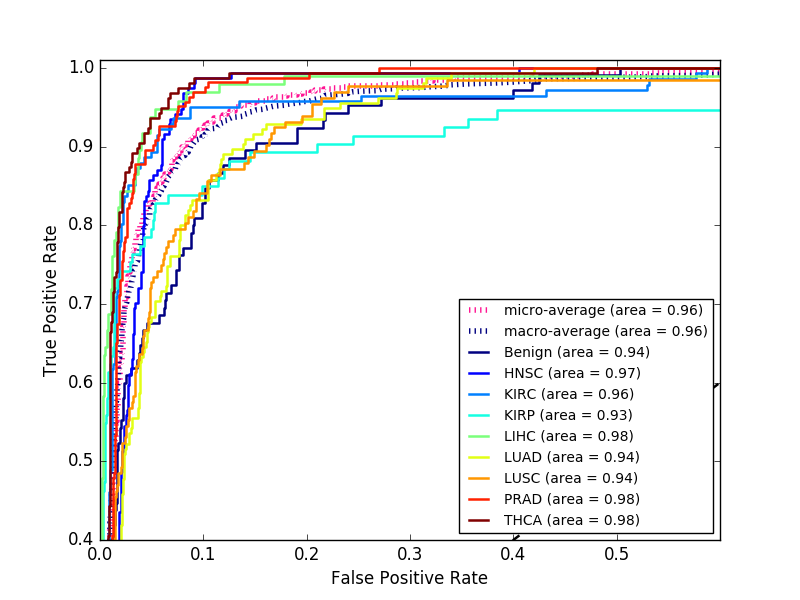
\includegraphics[width=\textwidth]{img/c_r/c_r_sdae_mlp_roc.png}
         \caption{}
     \end{subfigure}
     \begin{subfigure}[b]{0.49\textwidth}
         \centering
         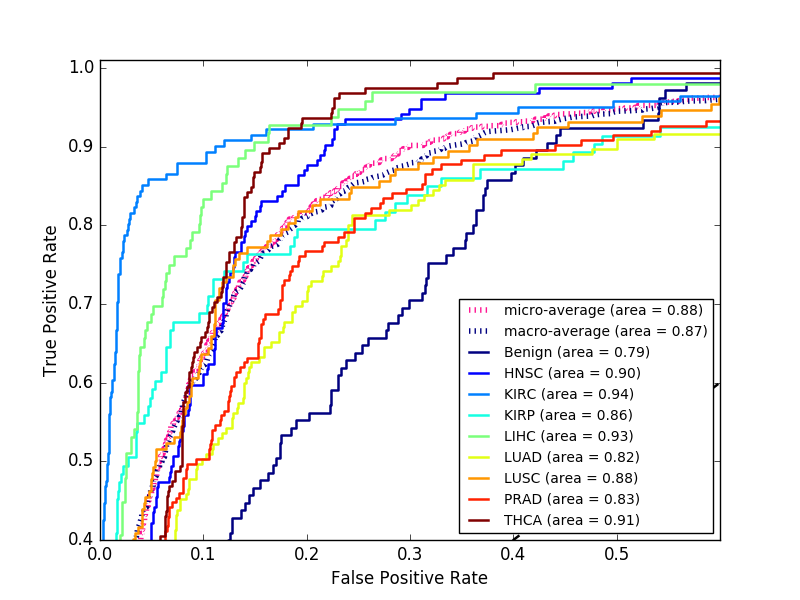
\includegraphics[width=\textwidth]{img/c_r/c_r_sdae_moe_roc.png}
         \caption{}
     \end{subfigure}
        \caption{CNV and RNA-seq SDAE bimodal model ROC plots for a) dGMU b) GMU c) MLP and d) ME.}
        \label{fig:c_r_sdae_roc}
\end{figure}

\begin{table}[H]
   \caption{Summary of classification agreement for CNV and RNA-seq SDAE reduced to 500 features.} 
   \small % text size of table content
   \centering % center the table
   \begin{tabular}{lllll} % alignment of each column data
   \toprule[\heavyrulewidth]\toprule[\heavyrulewidth]
   \textbf{Modality} & \textbf{Accuracy} & \textbf{Precision} & \textbf{Recall} & \textbf{F1-score} \\ 
   \midrule
   \multicolumn{1}{l}{\textbf{Bimodal}} \\
        dGMU & 0.8764 &	0.8739 & 0.8749 & 0.8737\\
        GMU  & 0.8722 &	0.8700 & 0.8661 & 0.8675\\
        MoE  & 0.7611 &	0.7617 & 0.7566 & 0.7556\\
        MLP  & 0.8622 &	0.8613 & 0.8542 & 0.8570\\
        SVM  & 0.8605 &	0.8567 & 0.8542 & 0.8550\\
   \midrule
   \multicolumn{1}{l}{\textbf{CNV}} \\
        MLP  & 0.7586 &	0.7622 & 0.7534 & 0.7526\\
        SVM  & 0.7343 &	0.7459 & 0.7275 & 0.7321\\
   \midrule
   \multicolumn{1}{l}{\textbf{RNA-seq}}  \\
        MLP  & 0.8530 &	0.8560 & 0.8425 & 0.8477\\
        SVM  & 0.8429 &	0.8388 & 0.8347 & 0.8362\\
   \bottomrule[\heavyrulewidth] 
   \end{tabular}
   \label{table:c_r_sdae_exp41}
\end{table}

\begin{figure}[H]
     \centering
     \begin{subfigure}[b]{\textwidth}
         \centering
         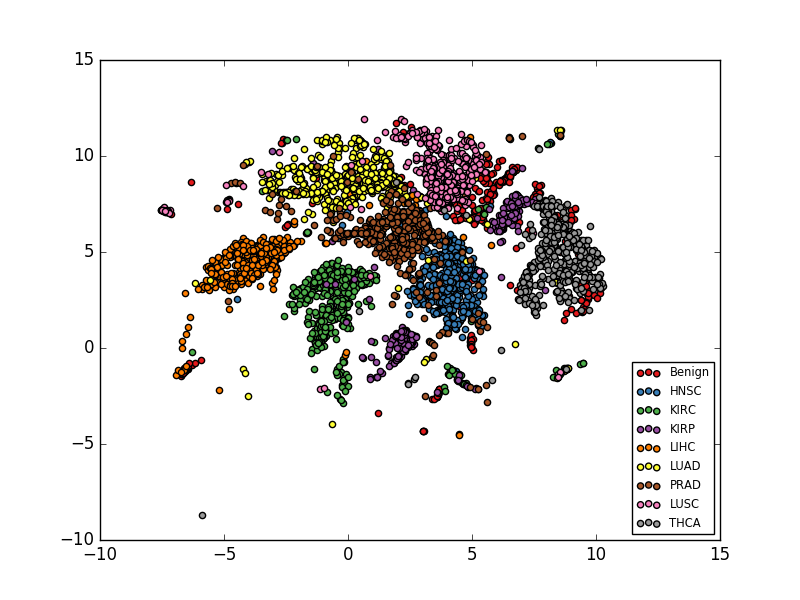
\includegraphics[width=\textwidth]{img/c_r/c_r_sdae_tsne.png}
     \end{subfigure}
        \caption{CNV and RNA-seq SDAE dGMU model latent space clustered with t-distributed stochastic neighbor embedding (t-SNE).}
        \label{fig:c_r_sdae_tsne}
\end{figure}

\subsubsection{DCF}

\begin{figure}[H]
     \centering
     \begin{subfigure}[b]{0.49\textwidth}
         \centering
         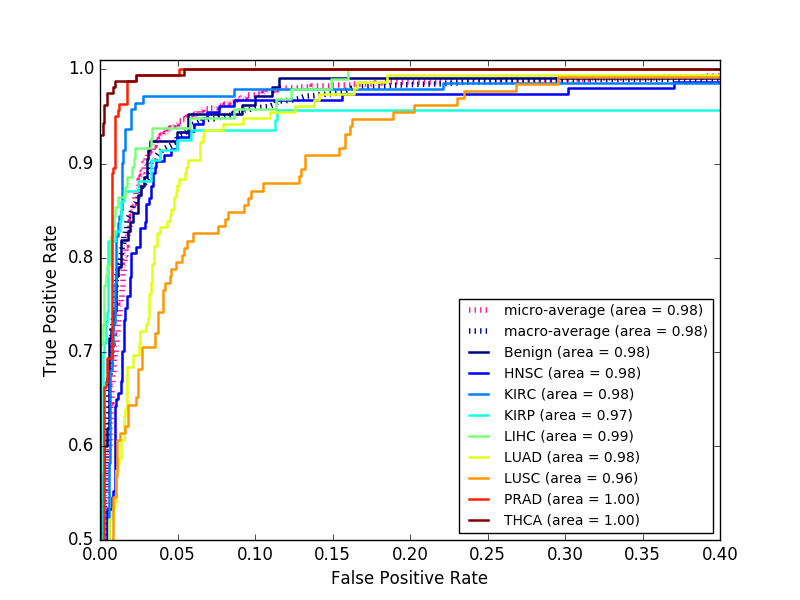
\includegraphics[width=\textwidth]{img/c_r/c_r_dcf_dgmu_roc.png}
         \caption{}
     \end{subfigure}
     \hfill
     \begin{subfigure}[b]{0.49\textwidth}
         \centering
         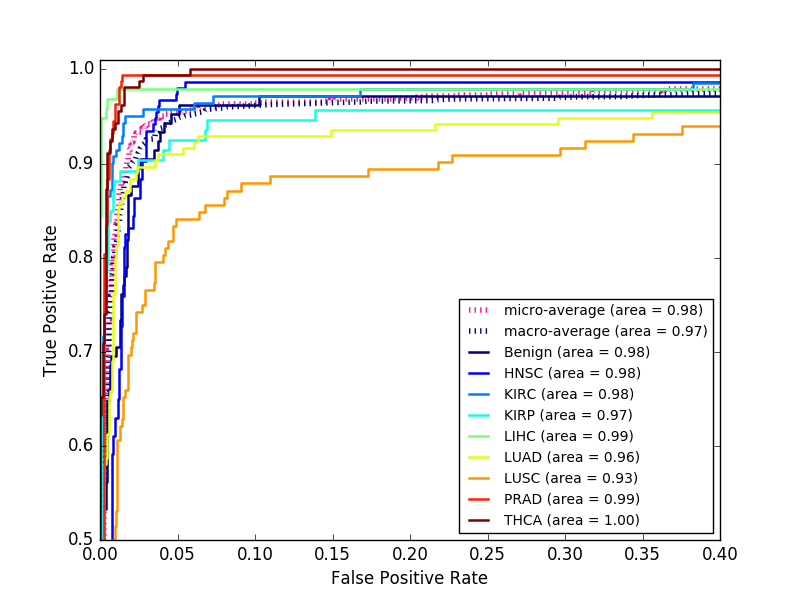
\includegraphics[width=\textwidth]{img/c_r/c_r_dcf_gmu_roc.png}
         \caption{}
     \end{subfigure}
     \hfill
     \begin{subfigure}[b]{0.49\textwidth}
         \centering
         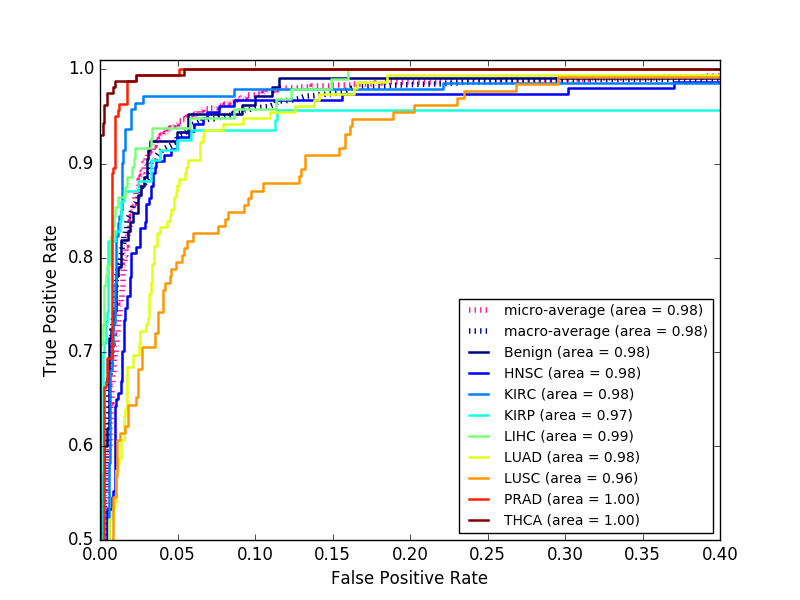
\includegraphics[width=\textwidth]{img/c_r/c_r_dcf_mlp_roc.png}
         \caption{}
     \end{subfigure}
     \begin{subfigure}[b]{0.49\textwidth}
         \centering
         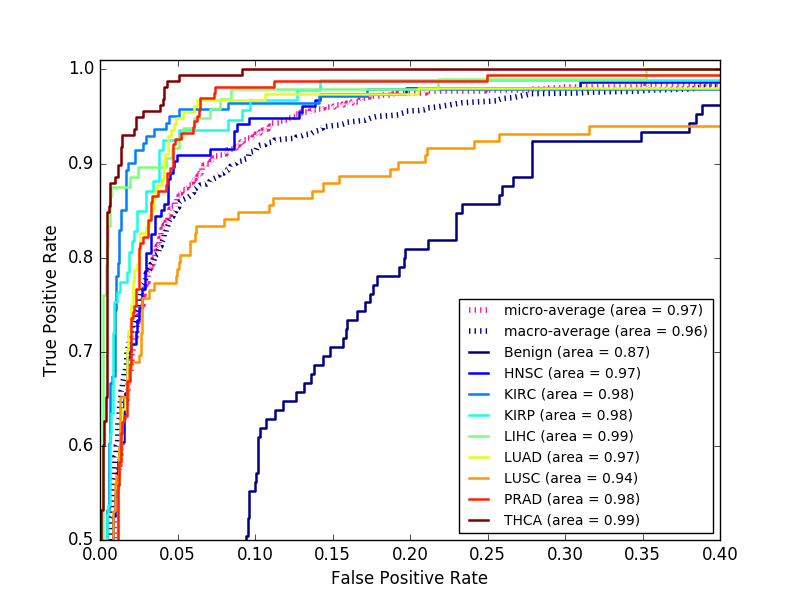
\includegraphics[width=\textwidth]{img/c_r/c_r_dcf_moe_roc.png}
         \caption{}
     \end{subfigure}
        \caption{CNV and RNA-seq DCF bimodal model ROC plots for a) dGMU b) GMU c) MLP and d) ME.}
        \label{fig:c_r_dcf_roc}
\end{figure}

\begin{figure}[H]
     \centering
     \begin{subfigure}[b]{\textwidth}
         \centering
         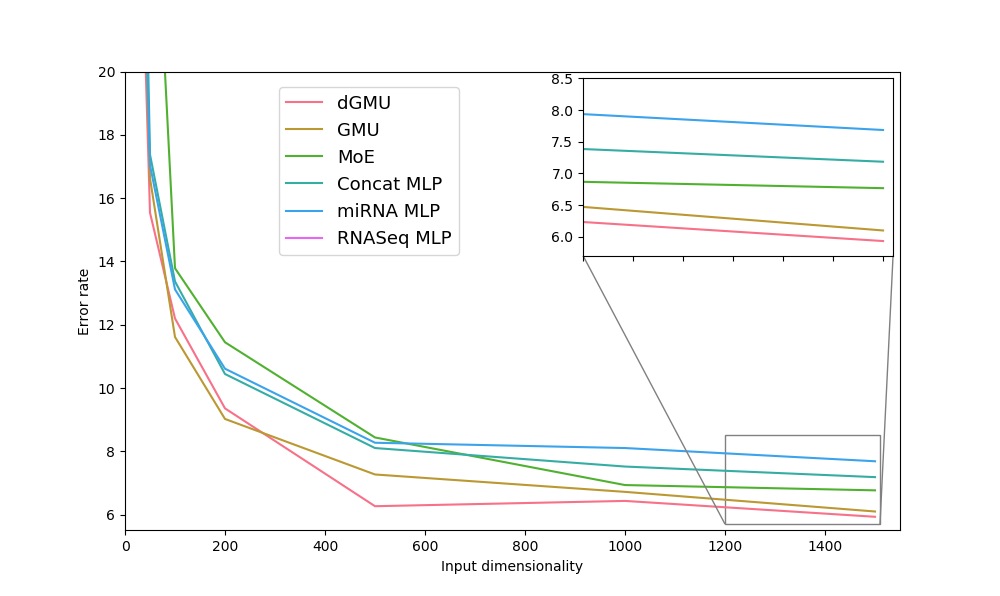
\includegraphics[width=\textwidth]{img/c_r/exp82.png}
     \end{subfigure}
        \caption{CNV and RNA-seq DE model error rates as a function of input dimensionality.}
        \label{fig:c_r_dcf_exp82}
\end{figure}

\begin{table}[H]
   \caption{Summary of classification agreement for CNV and RNA-seq DCF reduced to 500 features.} 
   \small % text size of table content
   \centering % center the table
   \begin{tabular}{lllll} % alignment of each column data
   \toprule[\heavyrulewidth]\toprule[\heavyrulewidth]
   \textbf{Modality} & \textbf{Accuracy} & \textbf{Precision} & \textbf{Recall} & \textbf{F1-score} \\ 
   \midrule
   \multicolumn{1}{l}{\textbf{Bimodal}} \\
        dGMU & 0.9373 &	0.9373 & 0.9373 & 0.9373\\
        GMU  & 0.9273 &	0.9273 & 0.9273 & 0.9273\\
        MoE  & 0.9156 &	0.9109 & 0.9111 & 0.9109\\
        MLP  & 0.9189 &	0.9199 & 0.9123 & 0.9154\\
        SVM  & 0.9172 &	0.9175 & 0.9150 & 0.9136\\
   \midrule
   \multicolumn{1}{l}{\textbf{CNV}} \\
        MLP  & 0.7468 &	0.7795 & 0.7270 & 0.7200\\
        SVM  & 0.7335 &	0.7460 & 0.7256 & 0.7310\\
   \midrule
   \multicolumn{1}{l}{\textbf{RNA-seq}}  \\
        MLP  & 0.9097 &	0.9118 & 0.9022 & 0.9052\\
        SVM  & 0.9072 &	0.9104 & 0.9045 & 0.9004\\
   \bottomrule[\heavyrulewidth] 
   \end{tabular}
   \label{table:c_r_dcf_exp41}
\end{table}

\begin{figure}[H]
     \centering
     \begin{subfigure}[b]{\textwidth}
         \centering
         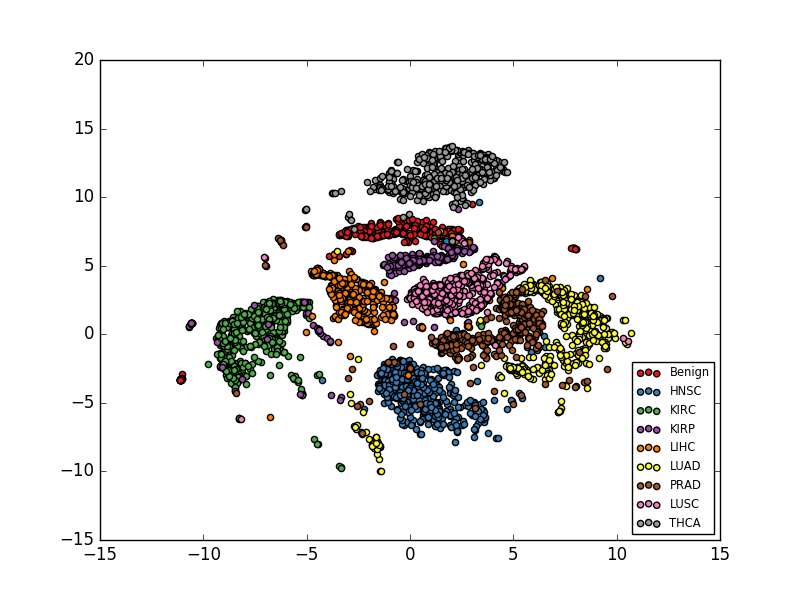
\includegraphics[width=\textwidth]{img/c_r/c_r_dcf_tsne.png}
     \end{subfigure}
        \caption{CNV and RNA-seq DCF dGMU model latent space clustered with t-distributed stochastic neighbor embedding (t-SNE).}
        \label{fig:c_r_dcf_tsne}
\end{figure}

%%%%%%%%%%%%%%%%%%%%%%%%%%%%%%%%%%%%%%%%%%%%%%%%%%%%%%%%%%%%%%%%%%%%%%%%%%%%%%%%%%
%M + S
%%%%%%%%%%%%%%%%%%%%%%%%%%%%%%%%%%%%%%%%%%%%%%%%%%%%%%%%%%%%%%%%%%%%%%%%%%%%%%%%%%

\subsection{miRNA-seq + SNV}\label{sub:m_s_results}

\subsubsection{SDAE}

\begin{figure}[H]
     \centering
     \begin{subfigure}[b]{0.49\textwidth}
         \centering
         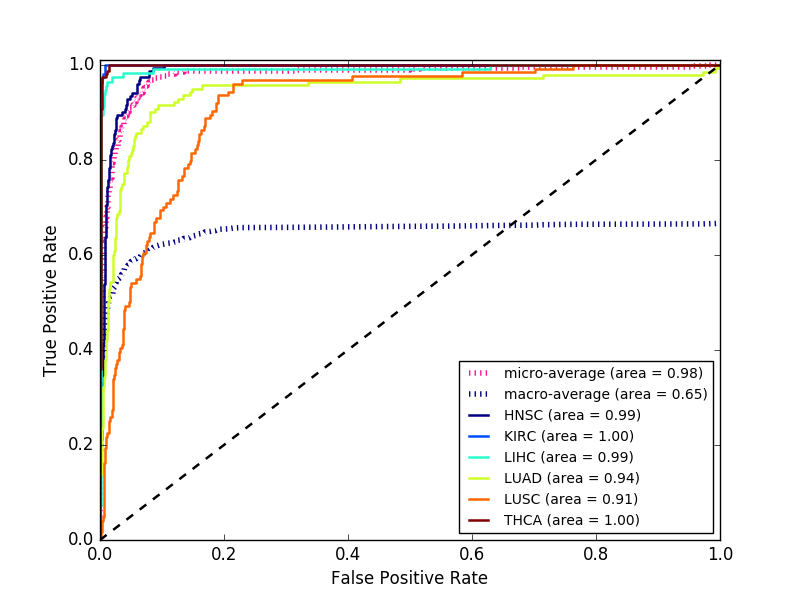
\includegraphics[width=\textwidth]{img/m_s/m_s_sdae_dgmu_roc.png}
         \caption{}
     \end{subfigure}
     \hfill
     \begin{subfigure}[b]{0.49\textwidth}
         \centering
         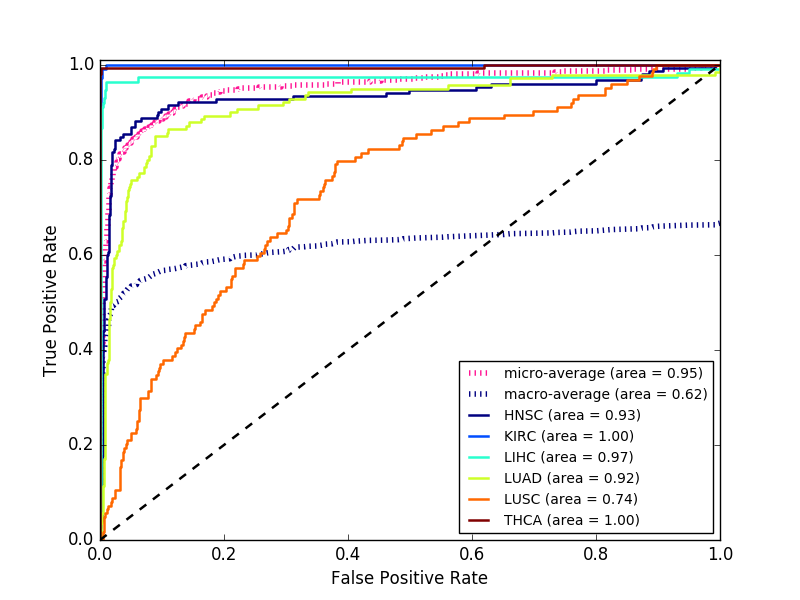
\includegraphics[width=\textwidth]{img/m_s/m_s_sdae_gmu_roc.png}
         \caption{}
     \end{subfigure}
     \hfill
     \begin{subfigure}[b]{0.49\textwidth}
         \centering
         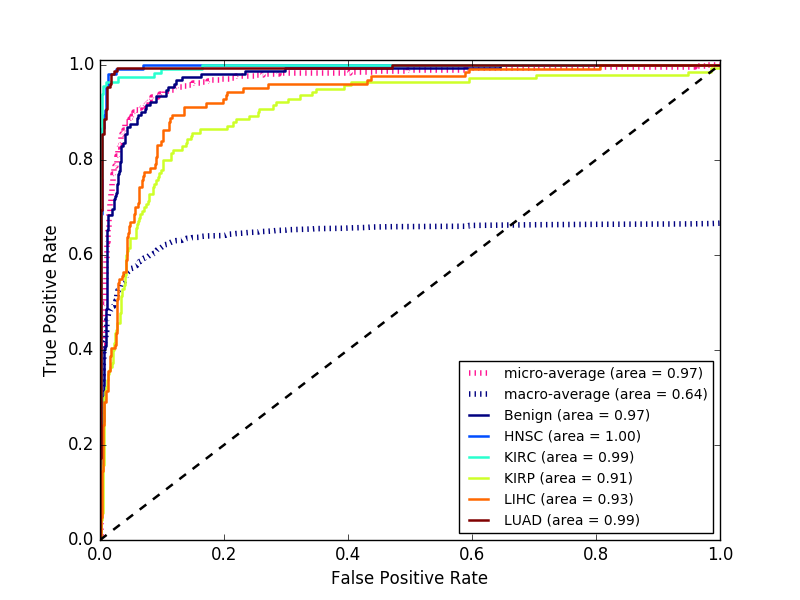
\includegraphics[width=\textwidth]{img/m_s/m_s_sdae_mlp_roc.png}
         \caption{}
     \end{subfigure}
     \begin{subfigure}[b]{0.49\textwidth}
         \centering
         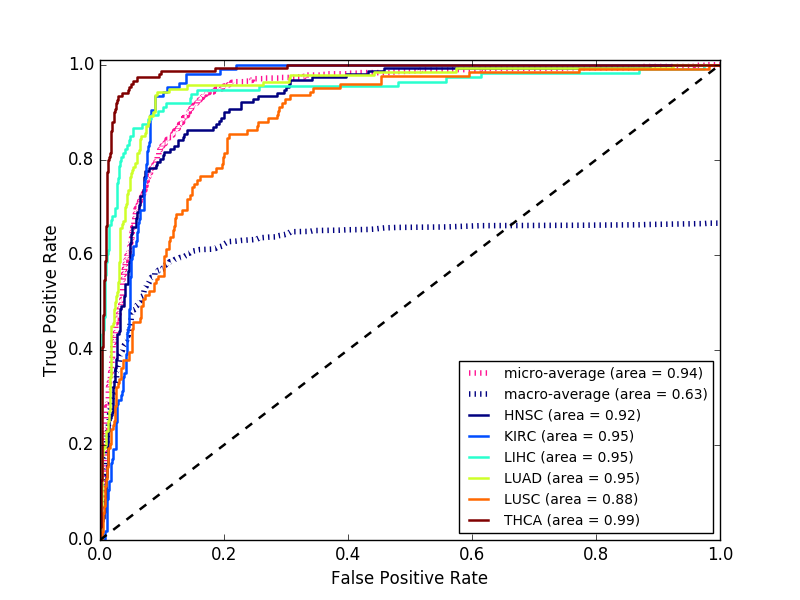
\includegraphics[width=\textwidth]{img/m_s/m_s_sdae_moe_roc.png}
         \caption{}
     \end{subfigure}
        \caption{miRNA-seq and SNV SDAE bimodal model ROC plots for a) dGMU b) GMU c) MLP and d) ME.}
        \label{fig:m_s_sdae_roc}
\end{figure}

\begin{table}[H]
   \caption{Summary of classification agreement for miRNA-seq and SNV SDAE reduced to 500 features.} 
   \small % text size of table content
   \centering % center the table
   \begin{tabular}{lllll} % alignment of each column data
   \toprule[\heavyrulewidth]\toprule[\heavyrulewidth]
   \textbf{Modality} & \textbf{Accuracy} & \textbf{Precision} & \textbf{Recall} & \textbf{F1-score} \\ 
   \midrule
   \multicolumn{1}{l}{\textbf{Bimodal}} \\
        dGMU & 0.9362 & 0.9375 & 0.9372 & 0.9373\\
        GMU  & 0.9260 & 0.9260 & 0.9260 & 0.9260\\
        MoE  & 0.9145 & 0.9199 & 0.9161 & 0.9173\\
        MLP  & 0.9222 & 0.9228 & 0.9227 & 0.9223\\
        SVM  & 0.9171 & 0.9198 & 0.9205 & 0.9199\\
   \midrule
   \multicolumn{1}{l}{\textbf{miRNA-seq}} \\
        MLP  & 0.9120 & 0.9207 & 0.9093 & 0.9113\\
        SVM  & 0.9107 & 0.9148 & 0.9134 & 0.9134\\
   \midrule
   \multicolumn{1}{l}{\textbf{SNV}}  \\
        MLP  & 0.6480 & 0.6454 & 0.6400 & 0.6407\\
        SVM  & 0.6173 & 0.6036 & 0.6013 & 0.6048\\
   \bottomrule[\heavyrulewidth] 
   \end{tabular}
   \label{table:c_r_sdae_summary}
\end{table}

\begin{figure}[H]
     \centering
     \begin{subfigure}[b]{\textwidth}
         \centering
         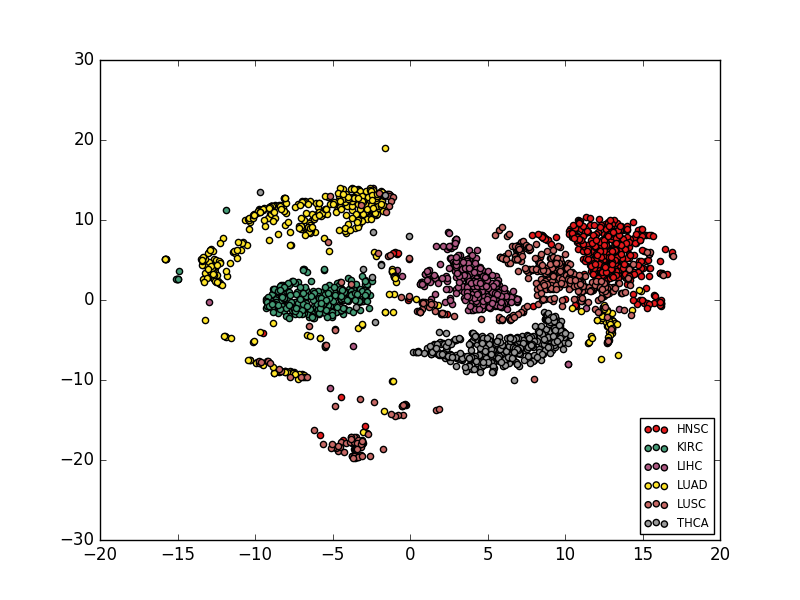
\includegraphics[width=\textwidth]{img/m_s/m_s_sdae_tsne.png}
     \end{subfigure}
        \caption{miRNA-seq and SNV SDAE dGMU model latent space clustered with t-distributed stochastic neighbor embedding (t-SNE).}
        \label{fig:m_s_sdae_tsne}
\end{figure}

\subsubsection{DCF}

\begin{figure}[H]
     \centering
     \begin{subfigure}[b]{0.49\textwidth}
         \centering
         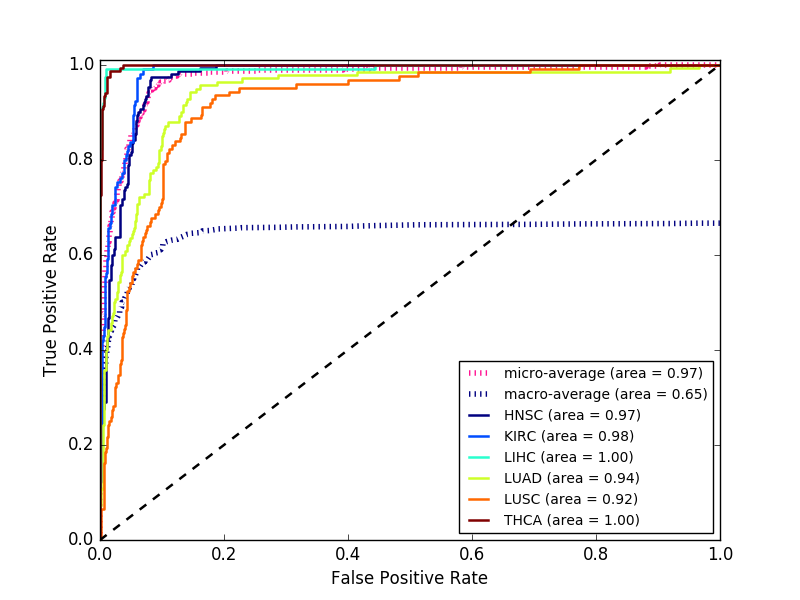
\includegraphics[width=\textwidth]{img/m_s/m_s_dcf_dgmu_roc.png}
         \caption{}
     \end{subfigure}
     \hfill
     \begin{subfigure}[b]{0.49\textwidth}
         \centering
         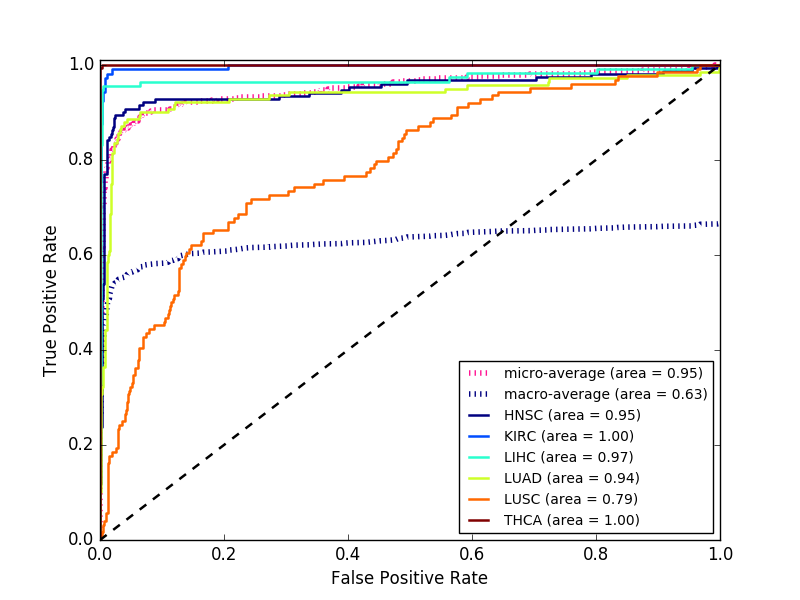
\includegraphics[width=\textwidth]{img/m_s/m_s_dcf_gmu_roc.png}
         \caption{}
     \end{subfigure}
     \hfill
     \begin{subfigure}[b]{0.49\textwidth}
         \centering
         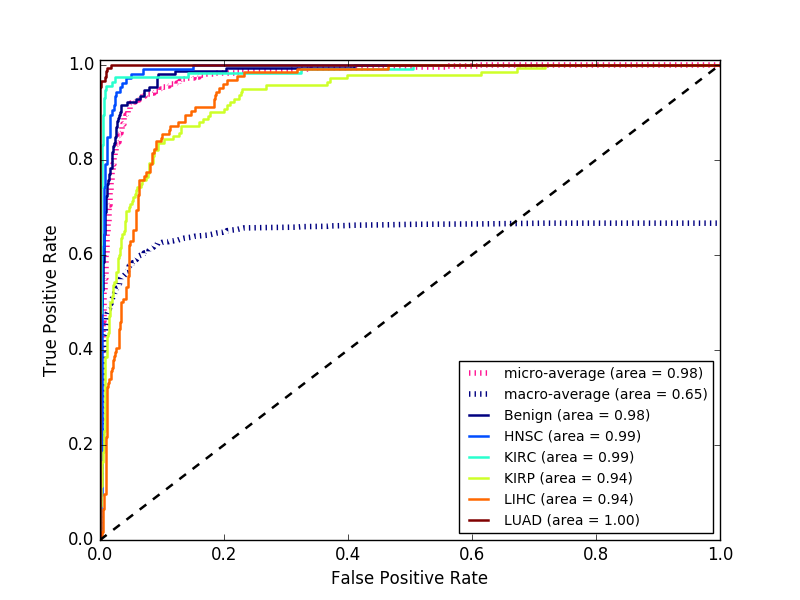
\includegraphics[width=\textwidth]{img/m_s/m_s_dcf_mlp_roc.png}
         \caption{}
     \end{subfigure}
     \begin{subfigure}[b]{0.49\textwidth}
         \centering
         \includegraphics[width=\textwidth]{img/m_s/m_s_dcf_moe_roc.png}
         \caption{}
     \end{subfigure}
        \caption{miRNA-seq and SNV DCF bimodal model ROC plots for a) dGMU b) GMU c) MLP and d) ME.}
        \label{fig:m_s_dcf_roc}
\end{figure}

\begin{figure}[H]
     \centering
     \begin{subfigure}[b]{\textwidth}
         \centering
         \includegraphics[width=\textwidth]{img/m_s/exp92.png}
     \end{subfigure}
        \caption{miRNA-seq and SNV DCF model error rates as a function of input dimensionality.}
        \label{fig:m_s_dcf_exp92}
\end{figure}

\begin{table}[H]
   \caption{Summary of classification agreement for miRNA-seq and SNV DCF reduced to 500 features.} 
   \small % text size of table content
   \centering % center the table
   \begin{tabular}{lllll} % alignment of each column data
   \toprule[\heavyrulewidth]\toprule[\heavyrulewidth]
   \textbf{Modality} & \textbf{Accuracy} & \textbf{Precision} & \textbf{Recall} & \textbf{F1-score} \\ 
   \midrule
   \multicolumn{1}{l}{\textbf{Bimodal}} \\
        dGMU & 0.9337 & 0.9358 & 0.9336 & 0.9334\\
        GMU  & 0.9324 & 0.9324 & 0.9324 & 0.9324\\
        MoE  & 0.9056 & 0.9067 & 0.9073 & 0.9070\\
        MLP  & 0.9120 & 0.9171 & 0.9154 & 0.9150\\
        SVM  & 0.8903 & 0.8921 & 0.8929 & 0.8924\\
   \midrule
   \multicolumn{1}{l}{\textbf{miRNA-seq}} \\
        MLP  & 0.9056 & 0.9073 & 0.9084 & 0.9077\\
        SVM  & 0.8980 & 0.8995 & 0.9006 & 0.8999\\
   \midrule
   \multicolumn{1}{l}{\textbf{SNV}}  \\
        MLP  & 0.5523 & 0.5834 & 0.5465 & 0.5512\\
        SVM  & 0.5599 & 0.5541 & 0.5561 & 0.5425\\
   \bottomrule[\heavyrulewidth] 
   \end{tabular}
   \label{table:m_s_dcf_summary}
\end{table}

\begin{figure}[H]
     \centering
     \begin{subfigure}[b]{\textwidth}
         \centering
         \includegraphics[width=\textwidth]{img/m_s/m_s_dcf_tsne.png}
     \end{subfigure}
        \caption{miRNA-seq and SNV DCF dGMU model latent space clustered with t-distributed stochastic neighbor embedding (t-SNE).}
        \label{fig:m_s_dcf_tsne}
\end{figure}
    
\backmatter{}
    \printbibliography



\end{document}

%TODO:
%Add official title page
%Explain backprop figure
%Explain what the percentage in the variant distribution figure is for
%Maybe add section to Summary of experimental dataset table in experimental results
%Make sure experimental dataset summary is in right order
%Add figure of the clustered latent spaces
